\documentclass{article}
\usepackage{float}
\usepackage{graphicx}
\usepackage{subfig}
\author{Simone Abelli, Stefano Azzone}
\title{DIMA Project report: MBox}
\begin{document}
\maketitle
\newpage
\tableofcontents
\newpage
\section{Introduction}
\subsection{Purpose}
The purpose of this document is to provide more technical and detailed
information about the mobile application developed. The Design Document is a
guide for the programmer that will manage the future development of the codebase
for the application in all its functions. The document will explain and motivate
all the architectural choices by providing a description of the components and
their interaction. We will also enforce the quality of the product through a set
of design characteristics. Finally we describe the implementation, integration
and test planning.
The topics touched by this document are:
\begin{itemize}
	\item high level architecture
	\item main components, screens and widgets
	\item runtime behavior
	\item design patterns
	\item more details on user interface
	\item requirements and their mapping on the architecture
	\item implementation and test planning
\end{itemize}

\subsection{Scope}
MBox is an application for mobile devices that allows users to access all the
music present on their devices without having to worry about manually managing 
the metadata. The target user has basic knowledge of the functions of the
mobile device (e.g. is able to interact with the filesystem). Since the
application is focused on users who want to listen to music, which is usually
done with a portable device, we will focus smartphones maily (the application
also works on tablets). For the development of this application we have decided
to use flutter since it's a framework thought for multiplatform deployment.

\subsection{Market analysis}
On Android and iOS there are many applications that allow the users to listen to
music present on the device or the respective app stores (e.g. Google Play Music
on Android, or the stock Music app on iOS). Nevertheless those applications do
not allow metadata management and some do not even allow to show lyrics when
present (e.g. Google Play Music).

From this point of view MBox is an evolution of existing music players since it
allows a simple and automatic metadata management. It automatically detects the
tracks present on the device and completes them with missing metadata,
a functionality that the competitors do not offer.

Moreover MBox also allows to look for other songs not present on the device, and
shows information about artist, albums and tracks.


\subsection{Glossary}
\paragraph{Queue:} a queue is a data structure containing a list of tracks
which are to be played according to a FIFO policy.
\paragraph{Metadata: } metadata are information of a track regarding the track
itself (e.g. track title, artist, album cover \ldots)

\newpage

\section{Description and requirements}
\subsection{Product description}
MBox has all the functionalities of a music player:
\begin{itemize}
    \item Detect music present in the Music folder
    \item Allow management of playlists
    \item Organize music by artist, album and playlist
    \item Allow to arrange tracks in a playback queue
    \item Play tracks (in random order if desired)
    \item Visualize metadata related to tracks
\end{itemize}
In addition to this, MBox allows a more advanced and automated metadata
management, and the access to other music information:
\begin{itemize}
    \item Automatically set missing metadata (Title, Artist, Album, Cover,
        Lyrics, Track number, Artist image, \ldots)
    \item Manually edit metadata
    \item Visualize information about artists like a brief description, albums
        and other songs
    \item Search on the internet for other songs and listen to them
\end{itemize}

\subsection{Assumptions}
\begin{itemize}
    \item When downloading metadata or looking for other music, internet
        connection is available
    \item The user is able to move their music to the Music folder
    \item The tracks are present on Spotify to download metadata
    \item When the user looks for a track not present on their device, it must
        be present on YouTube
    \item The tracks are in mp3 format (otherwise metadata management is harder)
    \item The access to the filesystem is granted
    \item The device on which the application is used has some means to 
        play music
\end{itemize}

\subsection{Functional requirements}
\begin{enumerate}
    \item The application can access the filesystem and fetch songs from the
        music folder
    \item The application can play the selected tracks
    \item The application allows the user to add or remove tracks from the
        playback queue
    \item The application allows the user to pause and resume playback
    \item The application allows the user to skip tracks in the queue
    \item The application should save the queue state to resume playback if the
        application is closed
    \item The application allows the user to add or remove playlists
    \item The application allows the user to add or remove tracks from playlists
    \item The application organizes the tracks by artist and album
    \item The application allows the user to view lyrics of currently playing 
        track
    \item The application allows the user to edit metadata of the tracks
    \item The application automatically adds missing metadata using an external
        service (in our case Spotify); already present metadata is kept
    \item The application can show information about the artists of the tracks
        present on the device (such as all their albums and tracks)
    \item The application allows the user to search for tracks not present on
        their device, and play them through an external service (in our case
        YouTube)
    \item It should be possible to use the application without an internet
        connection, obviously with limited functionalities (no external song
        search, metadata editing \ldots)
\end{enumerate}

\subsection{Non functional requirements}
\begin{enumerate}
    \item The application should feel snappy and responsive
    \item The application layout should be intuitive to use
    \item The application should be reliable
\end{enumerate}
\newpage

\section{Architectural Design}
\subsection{Architectural Style}
The application is logically subdivided in a frontend and a backend.
The frontend presents the information to the user and allows them to interact
with the backend. The backend contains and manages all the data and interfaces
with the external services.
\subsubsection{Frontend}

\begin{figure}[H]
	\noindent
	\makebox[\textwidth]{ 
		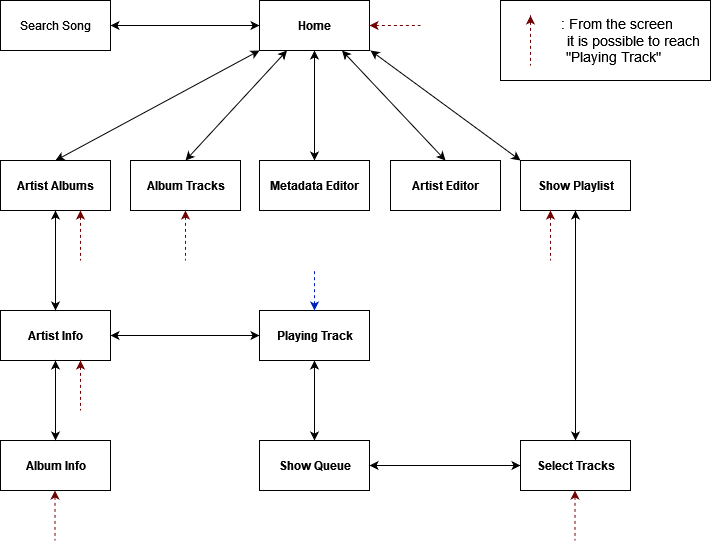
\includegraphics[scale=0.6]{images/ScreensDiagram.png}}
	\caption{Frontend system architecture} 
\end{figure}

The frontend is composed by the screens of the application. Once opened MBox
shows the \textbf{Home} screen. The Home screen is composed by 4 tabs:
\begin{itemize}
    \item \textit{Tracks}: a list of the tracks in alphabetical order; by
        selecting one we switch to the \textbf{PlayingTrack} screen, and start
        playing that track.
    \item \textit{Albums}: a list of the albums in alphabetical order; by
        selecting one we switch to the \textbf{AlbumTracks} screen, where we can
        select a track to play. 
    \item \textit{Artists}: a list of the artists in alphabetical order; by
        selecting one we switch to the \textbf{AlbumArtists} screen, where  we
        can select an album to show.
    \item \textit{Playlists}: a list of the playlists in alphabetical order; by
        selecting one we switch to the \textbf{ShowPlaylist} screen, from which
        we can start the playback; in the Playlists tab it is also possible to
        add a new playlist or remove an existing one.
\end{itemize}

By keeping a track pressed it is possible to open a drop down menu with a few
entries:
\begin{itemize}
    \item \textit{Edit metadata}: switch to the \textbf{MetadataEditor} screen
        to modify the metadata of the track
    \item \textit{Add to queue}
    \item \textit{Add to playlist}
\end{itemize}

By keeping an artist pressed it is possible to switch to the
\textbf{ArtistEditor} screen in order to change its image.

By touching the magnifying glass in the top right corner of the application, it
is possible to reach the \textbf{SearchSong} screen that allows the user to look
for songs that are not present on their device, and play them through an
external service (in our case YouTube).
\\\\
From the \textbf{PlayingTrack} screen it is possible to:
\begin{itemize}
    \item \textit{pause} and \textit{resume} playback
    \item \textit{skip} forward and backward in the queue
    \item \textit{change playback position} of the currently playing track
    \item view the \textit{album cover} and the \textit{lyrics} of the currently
        playing song
    \item check the \textit{artist information} by switching to the
        \textbf{ArtistInfo} screen: this screen shows a brief description of the
        artist (from Wikipedia) and a list of their albums; by selecting one of
        these, the user is brought to the \textbf{AlbumInfo} screen, from which 
        they can view all the tracks and play them using YouTube
    \item \textit{show the queue} by switching to the \textbf{ShowQueue} screen.

\end{itemize}

The \textbf{ShowQueue} screen shows the current track queue; the tracks are
ordered according to their position in the queue, where the currently playing
track has index 0, the past tracks have negative index, and the future tracks
have positive index. From here it is possible to add new tracks to the queue by
means of the \textbf{SelectTracks} screen. Almost every screen has a
\textbf{PlayBar} that allows to pause and resume playback, and shows currently
playing track info and artwork. By pressing it, the user is brought back to the
\textbf{PlayingTrack} screen.

\subsubsection{Backend}
The backend is composed by various modules:
\begin{itemize}
    \item \textbf{Database}
    \item \textbf{Track queue}
    \item \textbf{Metadata loader}
    \item \textbf{Player}
    \item \textbf{Worker}
\end{itemize}

The database is the core of the application and all the other backend components
depend on it. Indeed the metadata loader is used by the database to collect data
from the internet, the Worker is an isolate that allows the database to load in
a parallel fashion data from internal storage, the track queue is initialized by
the database, and the player uses the information contained in the database to
play music.

\paragraph{Database}
The database is the main component of the application. This component is not an
actual database for the following reason: in our application most of the time we
want to fetch the data of a particular category (tracks, albums, artists,
playlists). The use of a real database for this reason would be superfluous: it
suffices for our purposes to use a hand crafted one.
\\
Moreover our database has other functionalities that are tightly coupled with
the domain's data and it would thus be difficult to integrate them in a
traditional one, and probably inefficient.
\\\\
When the appication boots, the database is initialized.
\\
It uses the worker isolate and the metadata loader to discover which tracks are
present on the device:
\begin{enumerate}
    \item Loads the saved database file (if it exists) with all its contents:
    tracks, artists, albums, playlist, current track queue.
    \item Checks the Music folder for songs not present in the database ile.
    \item For those songs the missing metadata, available on the internet, are
        downloaded and written in the music file (as id3 tag). 
    \item The new tracks are inserted in the database (along with its metadata).
    \item Update the database file.
\end{enumerate}
Once the database is initialized all the other components can access the music
data from it. 
\\\\
Another functionality of the database is to allow the user to modify the
metadata of the tracks. Finally this component also grants the user the ability
to refresh the database itself: all the data will be reloaded from scratch.

\paragraph{Track queue}
The track queue is the list of all the songs to be played. It is initialized and
saved by the database to grant persistency across application restart. An index
is assigned to each track: the track of index 0 is the one currently playing,
one with negative index has already been played, and one with positive index
will be played.
\\
Through the frontend components the user can modify the track queue, by adding,
removing tracks or changing the one currently playing.

\paragraph{Metadata loader}
The metadata loader is the component that handles the interaction with the
internet. It is capable of:
\begin{enumerate}
    \item Checking the internet connection.
    \item Retrieving and extracting track information from the Spotify api.
    \item Retrieving and extracting lyrics from the Genius api.
    \item Retrieving information about artists from Wikipedia.
    \item Searching for songs on YouTube.
\end{enumerate}
All these functions are used by the application to perform all its tasks.

\paragraph{Player}
The player is the component that allows music playback: it allows to pause or
resume a track, update the track position, go forward or backward in the track
queue. It automatically switches to the next song in queue when the current one
is over.
\\
It also informs the components interested when the currently playing song
changes.


\paragraph{Worker}
The worker is a component that includes an isolate and an interface to
communicate with it. The isolate is tasked with the management of the access to
the internal storage.
\\
It reads and writes database information. It is used to separate the access to
file from the main isolate, in order to increase performance.

\subsection{Architectural Patterns}

\subsubsection{Facade pattern}
In the system architecture we can notice that the user accesses the application
services through the frontend components; the frontend is the facade through
which the user accesses the internal logic of the system (the backend). In this
way it hides the internal complexity of the system, providing a simple and
unique interface that the user can access.

Using this pattern the user does not need to the internal structure of the
software and it can use the simple screens of the application to interact with
the backend. Another major benefit of this pattern is that any change in the
backend of the architecture will stay undetectable from the user, provided that
the facade stays the same.

For instance, if we decided to substitute the existing database with a SQL based
one, the user wouldn't notice a thing.

\subsubsection{Master-Worker pattern}
When the application boots an isolate is created. This isolate is a worker and
accepts orders from the main thread (the Master). The Worker component in fact
keeps waiting for a message from the Master, and when it receives one, it is
processed, and if a reply is needed, it is sent to the Master. The Worker then
resumes waiting for work.

\subsubsection{Singleton pattern}
Some of the components are to be intended as singletons: only one instance of
that particular component must exist at a time, and different calls to that
component must reach that unique instance. This is achieved through the
singleton pattern. In our application all the components of the backend
(database, track queue, metadata loader, worker, player) are singletons, since
it would be unreasonable to have more than one instance of each.

\subsection{Component view}
Here we display the main architecture of our application, and describe in detail
all of its subcomponents.

\subsubsection{Home}

\begin{figure}[H]
	\noindent
	\makebox[\textwidth]{ 
		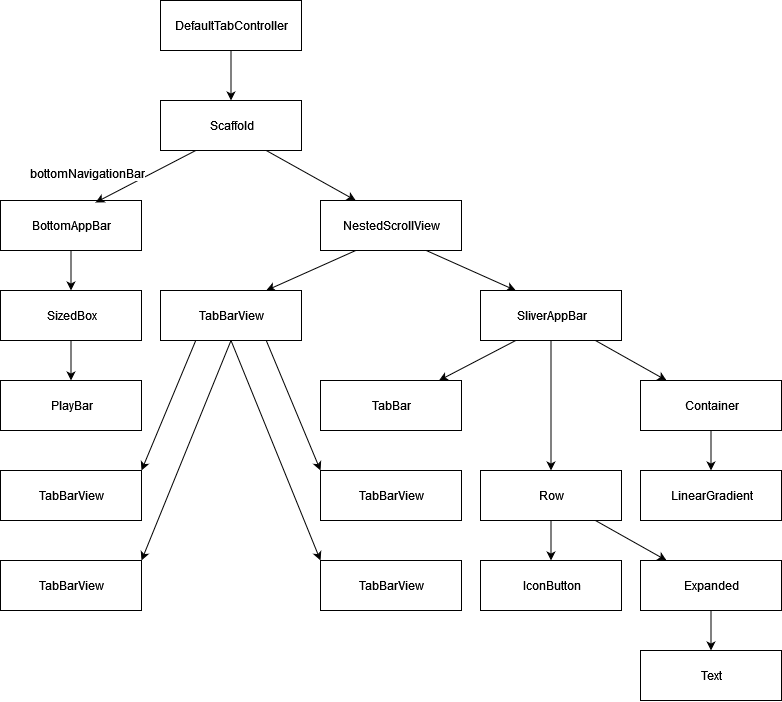
\includegraphics[scale=0.6]{images/Home.png}}
	\caption{Home} 
\end{figure}

The home component is the component shown when the application is first opened.
It is composed of the PlayBar, that allows to control playback and open the
track queue to modify it, and the NestedScrollView, that contains the TabBarView
and the SliverAppBar.

The TabBarView is the widget that shows the available
sections of the music library (TrackList, ArtistList, AlbumList and
PlaylistList).

The SliverAppBar contains the TabBar that actually allows to switch between the
available sections. It also hides itself when the TabBarView is scrolled down
for a sufficient amount.
 

\subsubsection{AlbumList}

\begin{figure}[H]
	\noindent
	\makebox[\textwidth]{ 
		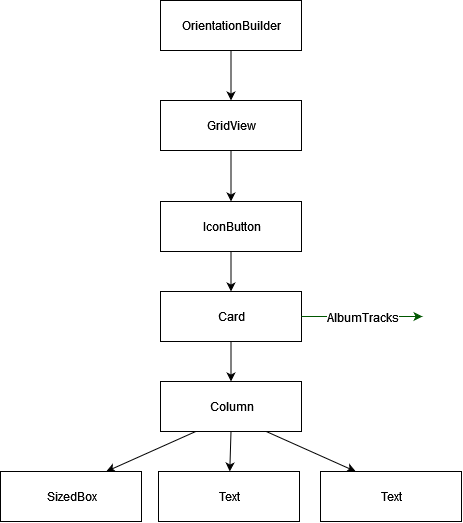
\includegraphics[scale=0.6]{images/AlbumList.png}}
	\caption{AlbumList} 
\end{figure}

This component displays in a grid (GridView) the list of albums (Card) present
on the device. The card contains the cover of the Album, its name and artist.

If a card is tapped (IconButton) the application navigates to the
tracklist of the selected album.

The OrientationBuilder allows to choose an appropriate layout for the device
orientation.

\subsubsection{ArtistList}

\begin{figure}[H]
	\noindent
	\makebox[\textwidth]{ 
		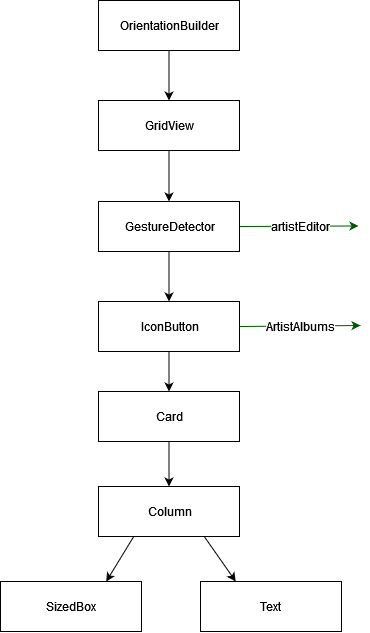
\includegraphics[scale=0.6]{images/ArtistList.png}}
	\caption{ArtistList} 
\end{figure}

This component displays a GridView of the Artist Cards, that contain the artist
name and image. The GestureDetector allows to edit the artist image through
ArtistEditor, while the IconButton allows to access the ArtistAlbum screen.

The OrientationBuilder allows to choose an appropriate layout for the device
orientation.

\subsubsection{PlaylistList}

\begin{figure}[H]
	\noindent
	\makebox[\textwidth]{ 
		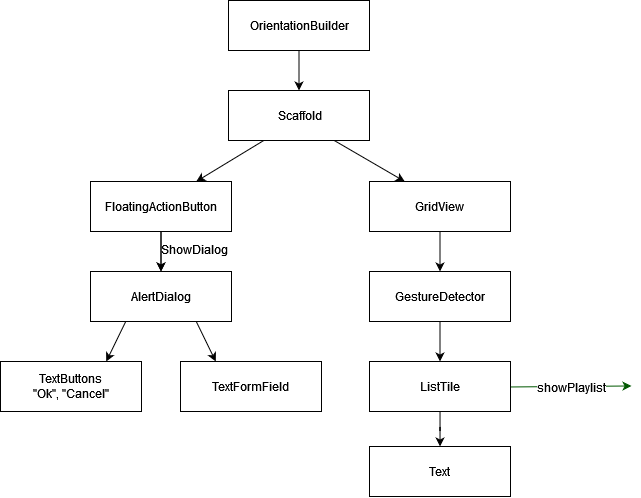
\includegraphics[scale=0.6]{images/PlaylistList.png}}
	\caption{PlaylistList} 
\end{figure}

This component displays a GridView of ListTiles. When tapped, the ListTile
navigates to the ShowPlaylist screen. The GestureDetector detects long presses
and shows accordingly a popup menu to delete the selected playlist if desired.

There is a FloatingActionButton in the bottom right corner of the screen that
allows creating new playlists.

The OrientationBuilder allows to choose an appropriate layout for the device
orientation.

\subsubsection{PlayBar}

\begin{figure}[H]
	\noindent
	\makebox[\textwidth]{ 
		\includegraphics[scale=0.5]{images/PlayBar.png}}
	\caption{PlayBar} 
\end{figure}

The PlayBar contains on the right a button that allow to play or pause music,
depending on current track queue state. On the left there is the description of
the currently playing track, with album cover, track name and artist.

When tapping the track description the application navigates to the PlayingTrack
screen.

\subsubsection{TrackList}

\begin{figure}[H]
	\noindent
	\makebox[\textwidth]{ 
		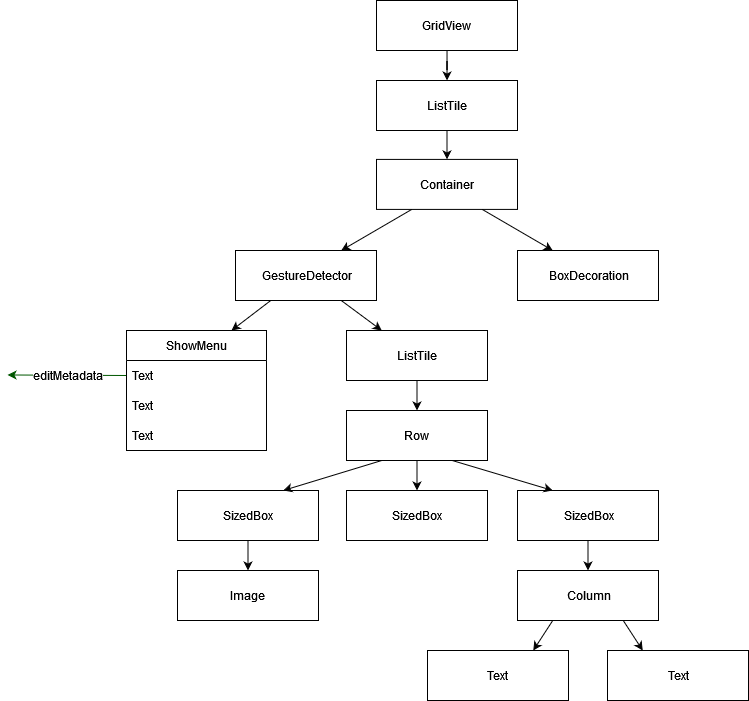
\includegraphics[scale=0.5]{images/TrackList.png}}
	\caption{TrackList} 
\end{figure}

The TrackList is the component that organizes tracks received as argument in a
grid. The grid is composed of GestureDetectors, longtapping which the popup menu
can be opened. 

The menu allows to execute operations on the selected track: view
its metadata, add it to queue or add it to playlist. Instead a short press on
the ListTile brings the user to the PlayingTrack screen and immediately starts
playing the track. 

The ListTile components have on the left the album cover, and
on the left the name and artist of the track.

\subsubsection{ProgressBar}

\begin{figure}[H]
	\noindent
	\makebox[\textwidth]{ 
		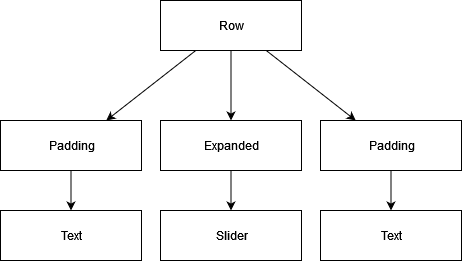
\includegraphics[scale=0.6]{images/ProgressBar.png}}
	\caption{ProgressBar} 
\end{figure}

The ProgressBar is the bar that allows monitoring the progress of the currently
playing track.

It also allows to move the track position forward or backward,
using the Slider. Text at the left side shows the track position, and at the
right shows the track length.

\subsubsection{CoverButton}

\begin{figure}[H]
	\noindent
	\makebox[\textwidth]{ 
		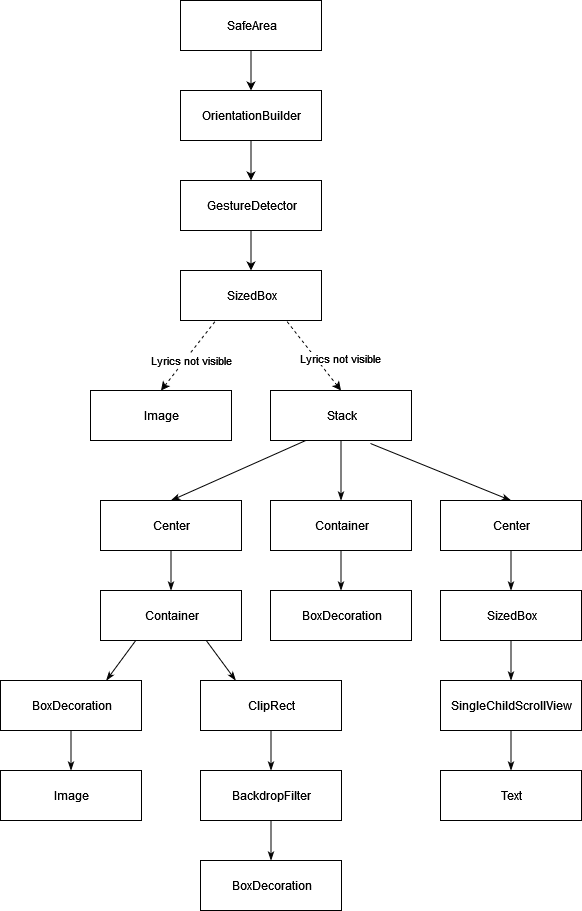
\includegraphics[scale=0.5]{images/CoverButton.png}}
	\caption{CoverButton} 
\end{figure}

The CoverButton is the widget that displays the cover art of an album inside the
PlayingTrack screen. If pressed (GestureDetector), it shows the lyrics
(scrollable Text) of the currently playing track, if available.

The background of the lyrics scroll view is transparent, so that the artwork can
be glimpsed behind them.

The CoverButton is subscribed to the Player, so that whenever a change in the
playing track occurs, that change is shown.

\subsubsection{ArtistEditor}

\begin{figure}[H]
	\noindent
	\makebox[\textwidth]{ 
		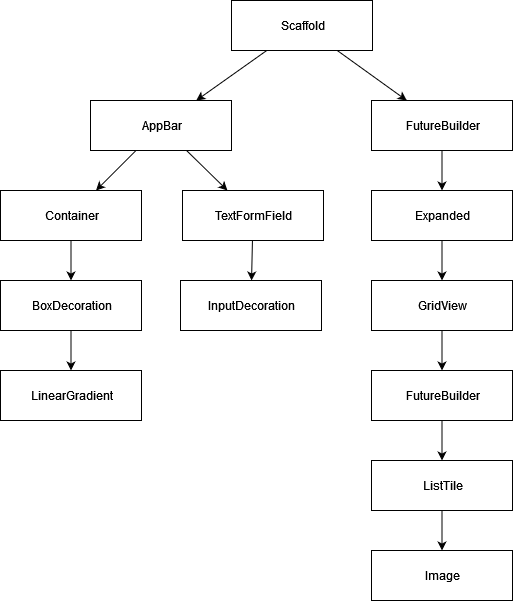
\includegraphics[scale=0.5]{images/ArtistEditor.png}}
	\caption{ArtistEditor} 
\end{figure}

The ArtistEditor is a widget that allows to select a new artwork for the input
artist. The artwork can be searched online by writing inside the TextFormField.

The results, if present, are listed as a grid (GridView) and returned by the
FutureBuilder, as tiles (ListTile) of images and names.

The LinearGradient widget allows to apply a pleasant color to the AppBar.

\subsubsection{MetadataEditor (also known as SearchSong)}

\begin{figure}[H]
	\noindent
	\makebox[\textwidth]{ 
		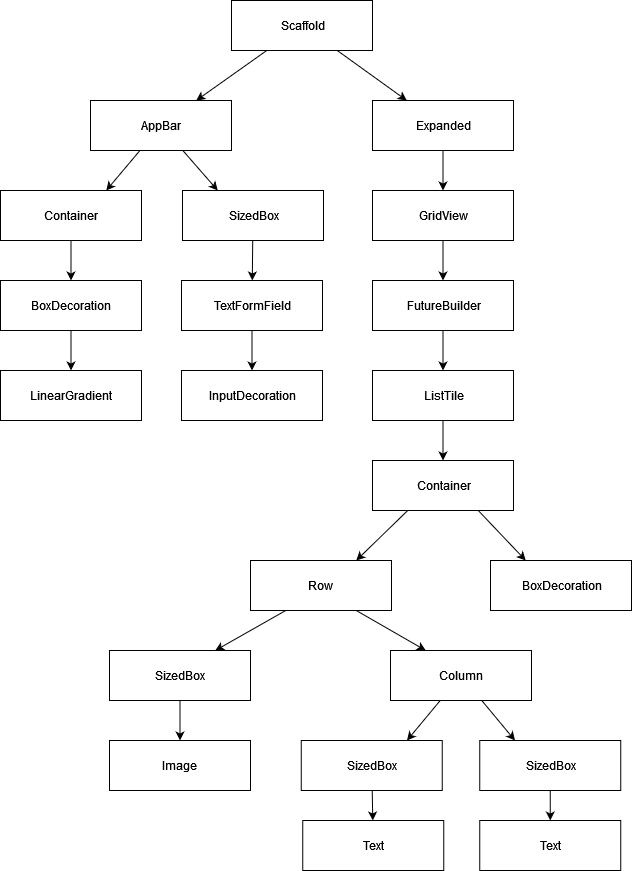
\includegraphics[scale=0.5]{images/MetadataEditor_SearchSong.png}}
	\caption{MetadataEditor (also known as SearchSong)} 
\end{figure}

The MetadataEditor is a widget that allows to set new metadata for the selected
track. The metadata can be searched online by writing inside the TextFormField.

The results, if present are returned as FutureBuilder and listed with a GridView
(this allows for flexible visualization in different orientations). They contain
image, name and artist. If tapped, the metadata of the selected track is
replaced with the metadata of the tapped track.

The LinearGradient widget allows to apply a pleasant color to the AppBar.

\subsubsection{AlbumInfo}

\begin{figure}[H]
	\noindent
	\makebox[\textwidth]{ 
		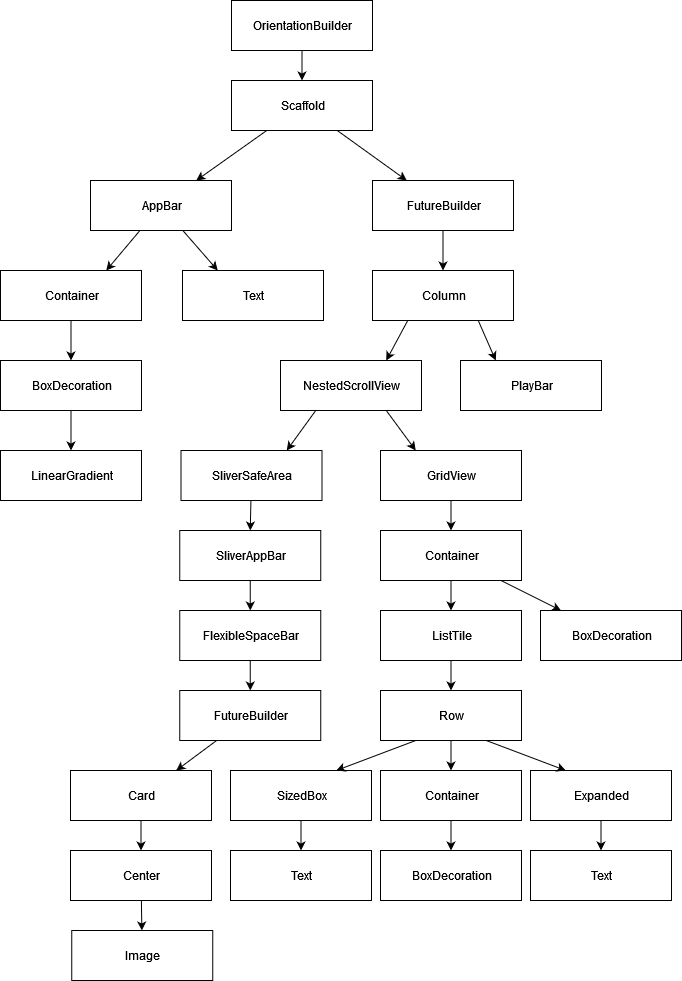
\includegraphics[scale=0.4]{images/AlbumInfo.png}}
	\caption{AlbumInfo} 
\end{figure}

The AlbumInfo screen is composed by the AppBar, the PlayBar and if available
(FutureBuilder), the info about the requested album.

The information about the album is contained in the NestedScrollView. At the top
we have a Card, showing the album cover. The cover will be hidden if scrolling
down the GridView. The grid is composed of tiles with track number and name.

\subsubsection{ArtistInfo}

\begin{figure}[H]
	\noindent
	\makebox[\textwidth]{ 
		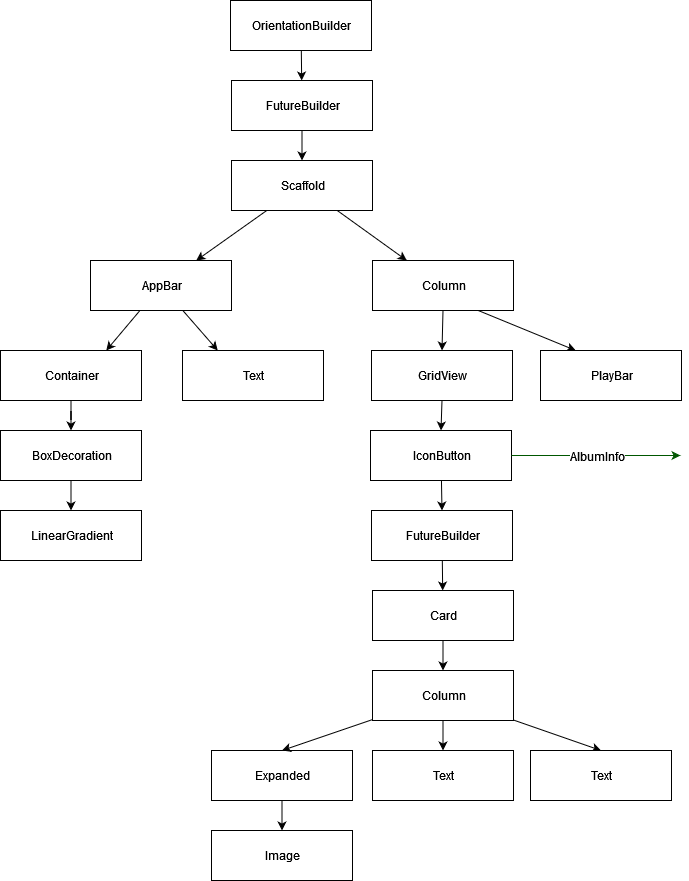
\includegraphics[scale=0.4]{images/ArtistInfo.png}}
	\caption{ArtistInfo} 
\end{figure}

The ArtistInfo screen is composed by the AppBar, the PlayBar and if available
(FutureBuilder), the info about the requested artist.

The information about the artist is contained in the NestedScrollView. The grid
is composed of cards with album image, name and artist.

\subsubsection{AlbumTracks}

\begin{figure}[H]
	\noindent
	\makebox[\textwidth]{ 
		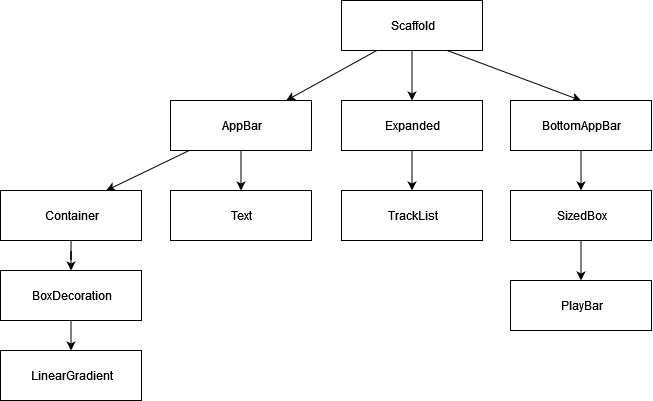
\includegraphics[scale=0.4]{images/AlbumTracks.png}}
	\caption{AlbumTracks} 
\end{figure}

The AlbumTracks screen is composed by the AppBar, the PlayBar and the TrackList.

It receives as input the list of tracks of an album, and displays them in a
grid by using the TrackList.

The first button of the grid instead allows to shuffle the album tracks, add
them to the queue and start playback.

\subsubsection{ArtistAlbums}

\begin{figure}[H]
	\noindent
	\makebox[\textwidth]{ 
		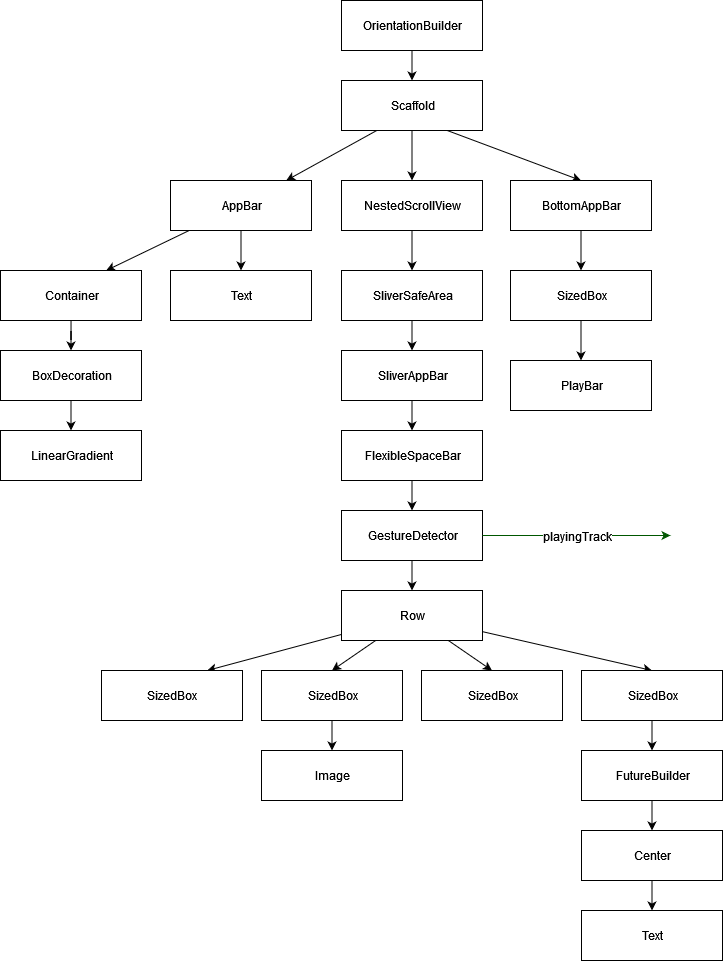
\includegraphics[scale=0.35]{images/ArtistAlbums.png}}
	\caption{ArtistAlbums}
\end{figure}

The ArtistAlbums screen is composed by:
\begin{itemize}
    \item the AppBar, that shows the name of the artist, 
    \item the PlayBar at the bottom, that allows controlling playback and
        accessing the queue with a tap,
    \item the albums of the selected artist organized in a grid; above it there
        is a card containing a small description of the artist and their image.
\end{itemize}

When tapping the card, the GestureDetector opens the ArtistInfo page of the
artist.

\subsubsection{PlayingTrack}

\begin{figure}[H]
	\noindent
	\makebox[\textwidth]{ 
		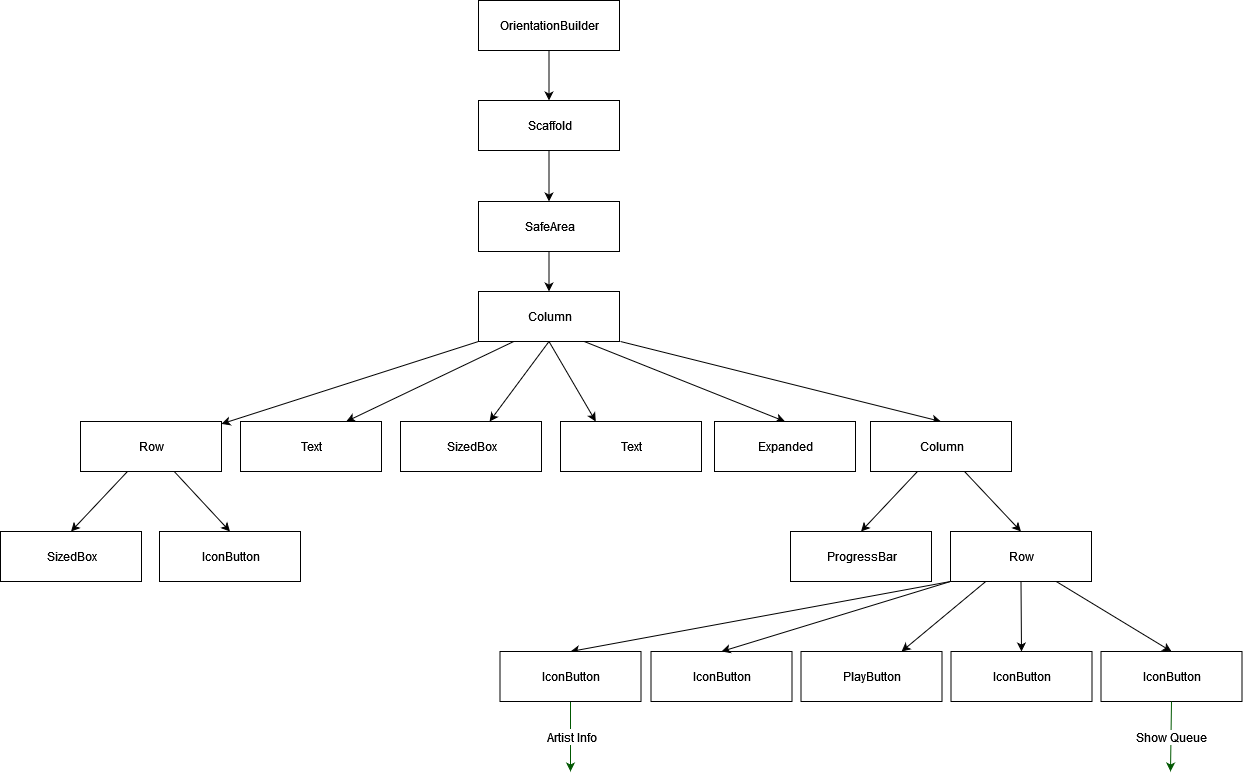
\includegraphics[scale=0.35]{images/PlayingTrack.png}}
	\caption{PlayingTrack}
\end{figure}

The PlayingTrack screen has a column composed of:
\begin{itemize}
    \item The track name and its artist
    \item The CoverButton that shows the album art of the current track, and If
        tapped the lyrics.
    \item The ProgressBar that shows the current position in the song.
    \item The Play/Pause, skip forward and backward, on the left the info button
        that shows the ArtistInfo screen, on the right the button to access the
        ShowQueue screen.
\end{itemize}

\subsubsection{SelectTracks}

\begin{figure}[H]
	\noindent
	\makebox[\textwidth]{ 
		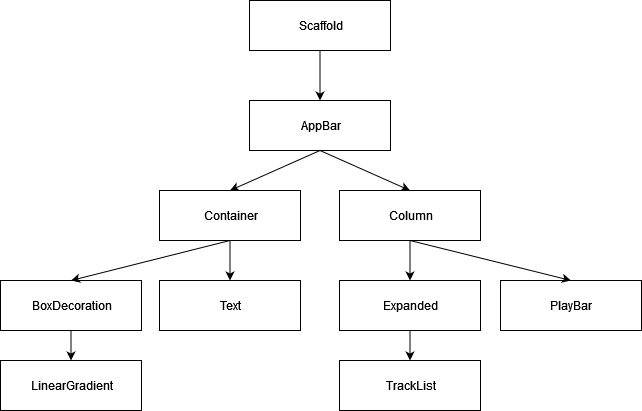
\includegraphics[scale=0.5]{images/SelectTracks.png}}
	\caption{SelectTracks}
\end{figure}

The SelectTracks screen is composed by a TrackList, and returns the tapped track
to the calling widget.

\subsubsection{ShowPlaylist}

\begin{figure}[H]
	\noindent
	\makebox[\textwidth]{ 
		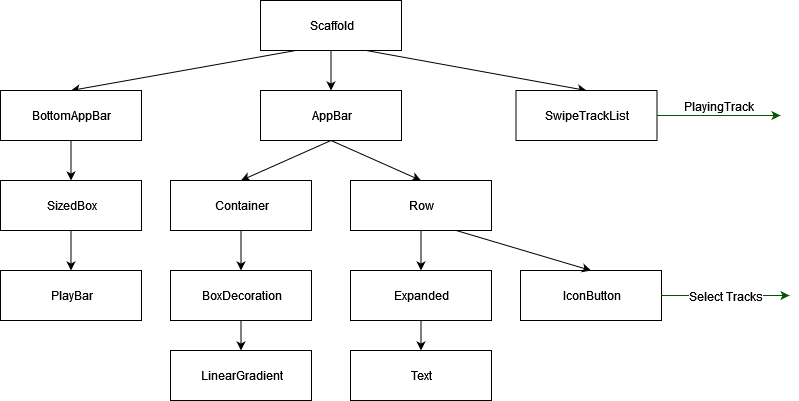
\includegraphics[scale=0.5]{images/ShowPlaylist.png}}
	\caption{ShowPlaylist}
\end{figure}

The ShowPlaylist screen is composed by:
\begin{itemize}
    \item the AppBar that contains the title of the selected playlist and the
        add button on the right, to add a track to the playlist through the
        SelectTracks screen.
    \item a SwipeTrackList that allows with a swipe to delete the swiped track,
        and is otherwise a normal TrackList.
    \item the PlayBar that allows to control music playback.
\end{itemize}

\subsubsection{ShowQueue}

\begin{figure}[H]
	\noindent
	\makebox[\textwidth]{ 
		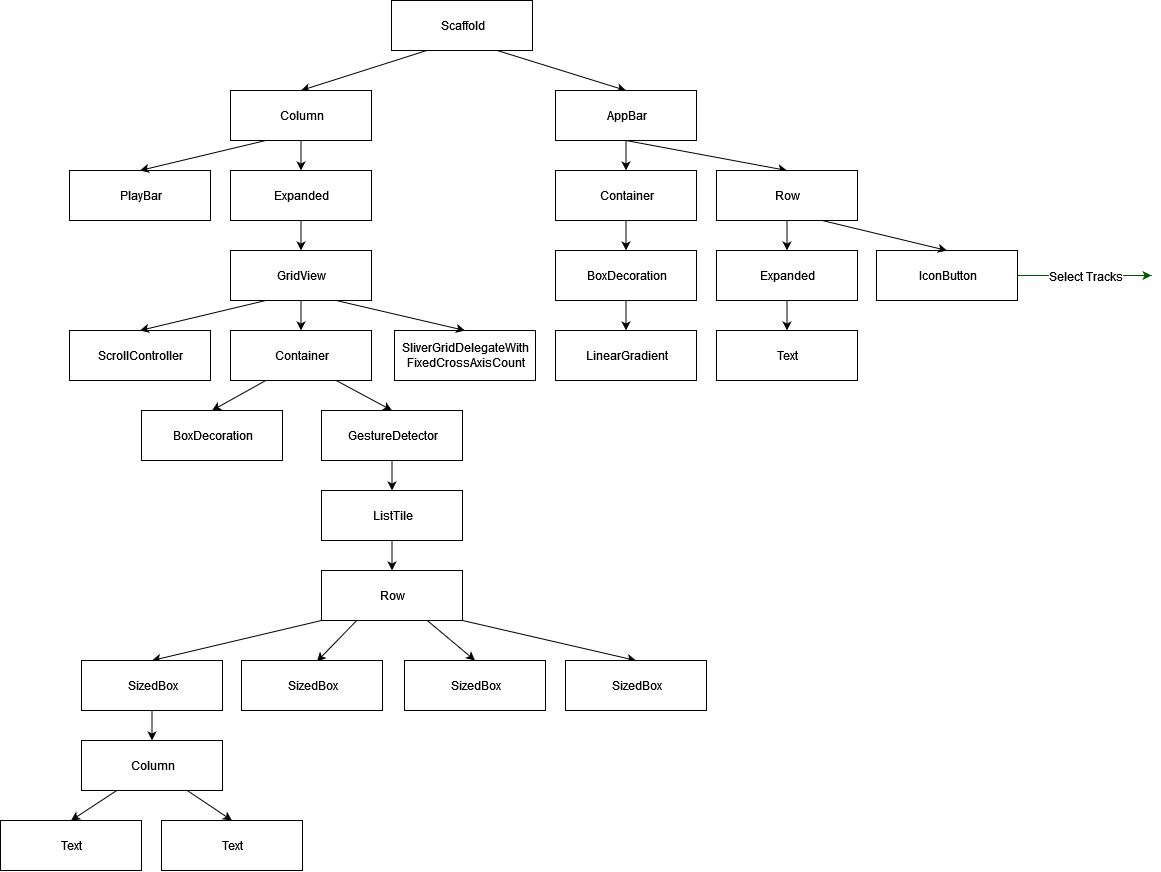
\includegraphics[scale=0.35]{images/ShowQueue.png}}
	\caption{ShowQueue}
\end{figure}

The ShowQueue screen is composed by:
\begin{itemize}
    \item the AppBar titled "Queue", and the
        add button on the right, to add a track to the queue through the
        SelectTracks screen.
    \item a Grid that lists the songs in the queue, composed by a number on the
        left that represent their position in the queue (0 if currently playing,
        greater than 0 if to be played, lesser than 0 if already played), the
        album art and track title and artist.

        By swiping one of the tracks it can be removed from the queue.
    \item the PlayBar that allows to control music playback.
\end{itemize}

\subsection{Deployment View}

The deployment of our software is completely bound to the smart device of the
user, with no additional hardware required (i.e. no need of servers/additional
internet infrastrucures to manage the service). 

\begin{figure}[H]
	\noindent
	\makebox[\textwidth]{ 
		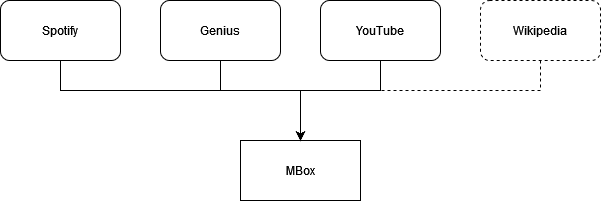
\includegraphics[scale=0.5]{images/Deployment.png}}
	\caption{Deployment view}
\end{figure}

Nevertheless for the correct usage of the application some external services are
actually required: 

\begin{itemize}
    \item Spotify is used to fetch the tracks' missing metadata
    \item Genius is used to find the lyrics of the songs, since this information
    is not provided by Spotify
    \item YouTube is used as a source of musical videos for the tracks not
    present on the storage of the device
    \item Wikipedia is used to get information about the artists
\end{itemize}

For what concerns the actual distribution of the software, as for most of the
mobile applications, we will use the usual app stores (e.g Google play store).

\newpage

\subsection{External Services}
The functionalities of the application are supported by a series of external
services:

\subsubsection{API}
\begin{itemize}
    \item \textbf{Spotify API}: when the application boots, tracks missing metadata are
    updated. If the ID3 tag containing the title of the song and the artist is
    available, it is used to obtain more information about the track (e.g. album
    cover, artist image). Otherwise the filename is used to determine the
    specific track.
    \item \textbf{Genius API}: provides the correct Genius page containing the lyrics;
    the lyrics are then extracted by the application.
    \item \textbf{YouTube}: we scrape the search page to get the link of the video, then
    the application that handles YouTube links will play that video.
    \item \textbf{Wikipedia API}: used to get the page of the artist.
\end{itemize}

\subsubsection{Libraries}
\begin{itemize}
    \item The \textbf{audioplayers} flutter library is able to play music given
    a path to the track.
    \item \textbf{audiotagger} is the only available flutter library able to
    read and write ID3 tags of mp3 files.
    \item \textbf{path\_provider} allows to find the path of the music folder and
    the database file.
    \item \textbf{crypto} for the hash function.
    \item \textbf{http} to fetch web pages.
    \item \textbf{html} to parse web pages.
    \item \textbf{url\_launcher} to launch YouTube links on the appropriate
    application.
    \item \textbf{permission\_handler} to ask and obtain internal storage
    permissions from the user.
    \item \textbf{image} for image handling.
\end{itemize}

\newpage

\section{User interface design}

The UI is composed by different screens that provide the user with a way to
interact with the system. In this section we present some screenshots that show
how the screens look like along with a brief description of how the user can
navigate between the screens.
\\\\
The interface is intuitive, simple to use, and it does not require the user to
read a manual.

\subsection{Screens description}
When the application is opened, the first screen shown is the Home page, that
contains a list of tabs.
\\\\
The first tab (\textit{image a}) shows all the tracks present on the device in a list. By
tapping on one of the tracks the playback starts and the app navigates to the
PlayingTrack screen (\textit{image f}). By tapping on the magnifying
glass on the upper right corner of the screen, the user is presented with a way
to search for tracks not present on the device and if desired play them through
an external service (\textit{image o}). Long tapping a track (\textit{image b}) opens
a dropdown menu with three options: the user can add the song to an existing
playlist, to the queue, or change its metadata.
\\\\
The second tab (\textit{image c}) contains the albums. Tapping on an album, the app
navigates to the AlbumTracks screen (\textit{image j}), that allows to pick a track to
play from the album or shuffle the tracks and play them.
\\\\
The third tab (\textit{image d}) containst the artists.  By long pressing the image of an
artist it is possible to change it. Tapping on an artist icon opens the
ArtistAlbums (\textit{image k}) screen, that provides some information about the artist
and allows selecting one of the albums by that artist.
\\\\
The fourth and last tab (\textit{image e}) shows the playlists. A new playlist can be
created by tapping the plus button in the lower right corner of the screen. By
tapping one of the existing playlists the user can view the contents of it in
the ShowPlaylist screen (\textit{image l}). Long pressing a playlist it is possible to
delete it.
\\\\
In all these tabs, at the very bottom of the screen, if there is at least a song
in the queue, a bar is shown. This bar shows the current song artwork, title and
artist, and allows to pause or resume playback. By tapping the bar itself, the
PlayingTrack (\textit{image f}) screen is shown.
\\\\
In the PlayingTrack screen (\textit{image f}), the user is shown the track name, artist
and cover. They can see the current playback progress and change it by
dragging the slider. On the very bottom of the screen there are, in order from
left to right: the ArtistInfo button, the previous track button, the play/pause
button, the next track button, the ShowQueue button.
By tapping on the cover the lyrics of the current song are shown (\textit{image g}).
\\\\
In the ArtistInfo screen (\textit{image h}) the user can see all the albums from the
artist (also those not present on the device). Selecting one of the albums, the
AlbumInfo screen is shown (\textit{image i}). Here the cover of that album and its tracks
are provided. By tapping on one of those tracks, the user can listen to them on
YouTube.
\\\\
The ShowPlaylist screen (\textit{image l}) lists the tracks present in a playlist. By
selecting one, all the tracks in the playlist will be added to the queue and the
selected track will be played. By pressing the shuffle button the tracks are
played in random order. The plus button on the top right corner allows to add
new tracks to the playlist. The user can easily remove a track from the playlist
by swiping right.
\\\\
The ShowQueue screen (\textit{image n}) lists all the tracks in the queue, sorted by
playback order. The plus button on the top right corner allows to add new tracks
to the queue. The user can easily remove a track from the queue by swiping
right. 
\\\\
The SelectTracks screen (\textit{image m}) is reached either from the ShowPlaylist or
from the ShowQueue screens to add tracks. A list of the tracks is provided, and
by tapping one, it is added to the playlist/queue.
\\\\
The EditMetadata and SearchTrack screens (\textit{image o}) look very similar. They
both have a search bar on which the user can type their query, and they provide
a list of results, from which it is possible to select one. In the latter screen
the selected track is opened on YouTube, while in the former the metadata of the
song to be changed are replaced with the new ones.
\\\\
When the device is in landscape mode, there are slight changes to the UI (\textit{images
q to v}): for example the lists of tracks become grids with two columns, and
the grids of albums and artists have two additional columns.

\subsection{Screenshots}

\setlength{\tabcolsep}{40pt}
\begin{figure}[H]
    \begin{tabular}{cc}
    \subfloat[Tracks scrolled]{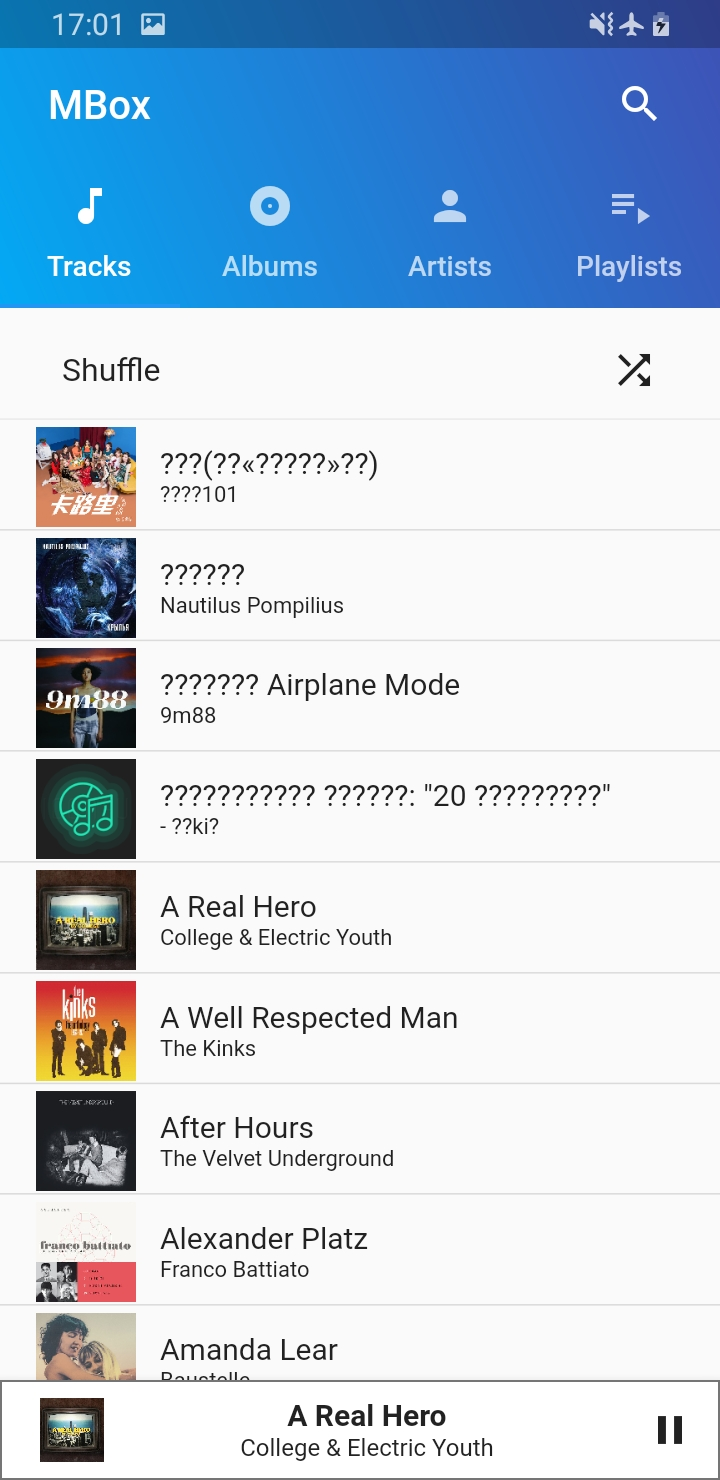
\includegraphics[width = 1.5in]{screens/1. Tracks.jpg}} &
    \subfloat[Tracks]{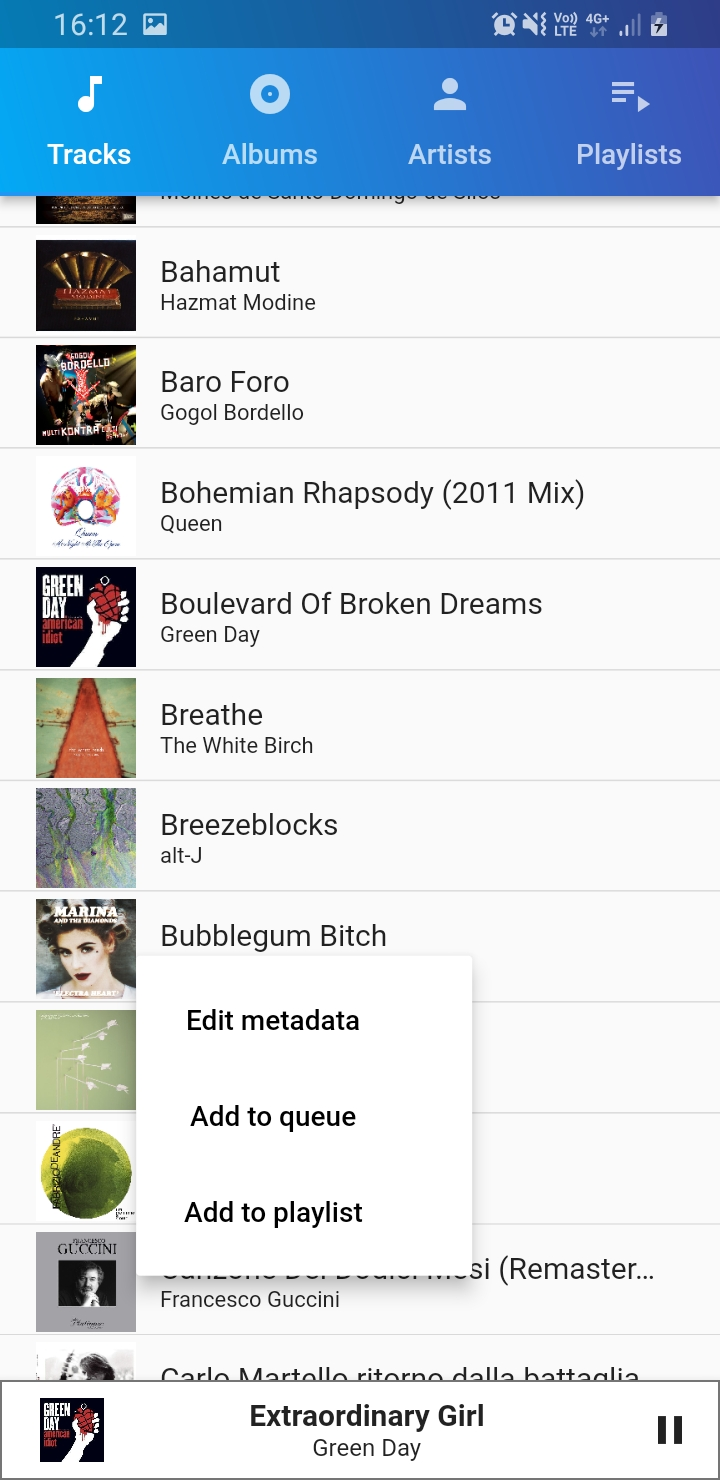
\includegraphics[width = 1.5in]{screens/2. Tracks_dropdown.jpg}}\\
    \\\\
    \subfloat[Albums]{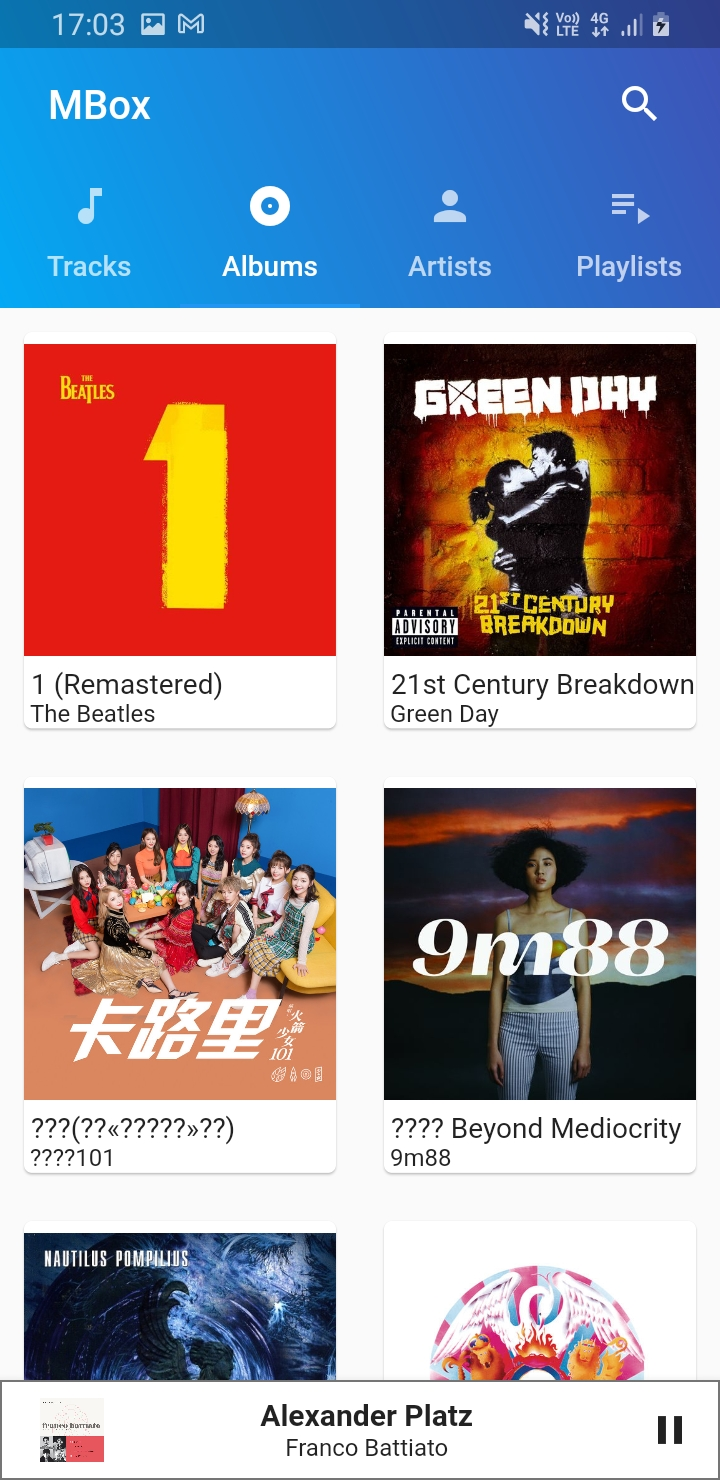
\includegraphics[width = 1.5in]{screens/3. Albums.jpg}} &
    \subfloat[Artists]{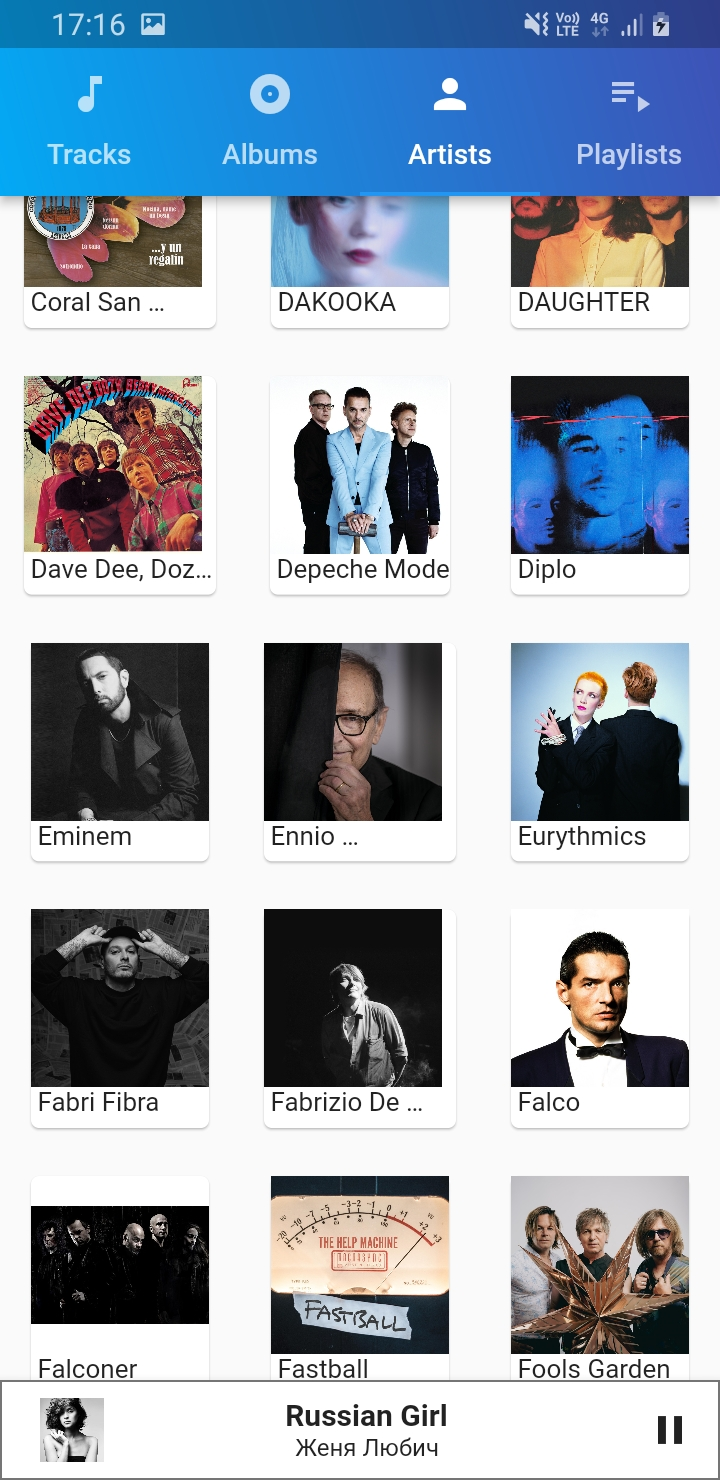
\includegraphics[width = 1.5in]{screens/4. Artists.jpg}}
    \end{tabular} 
\end{figure}

\newpage
\begin{figure}[H]
    \begin{tabular}{cc}
    \subfloat[Playlists]{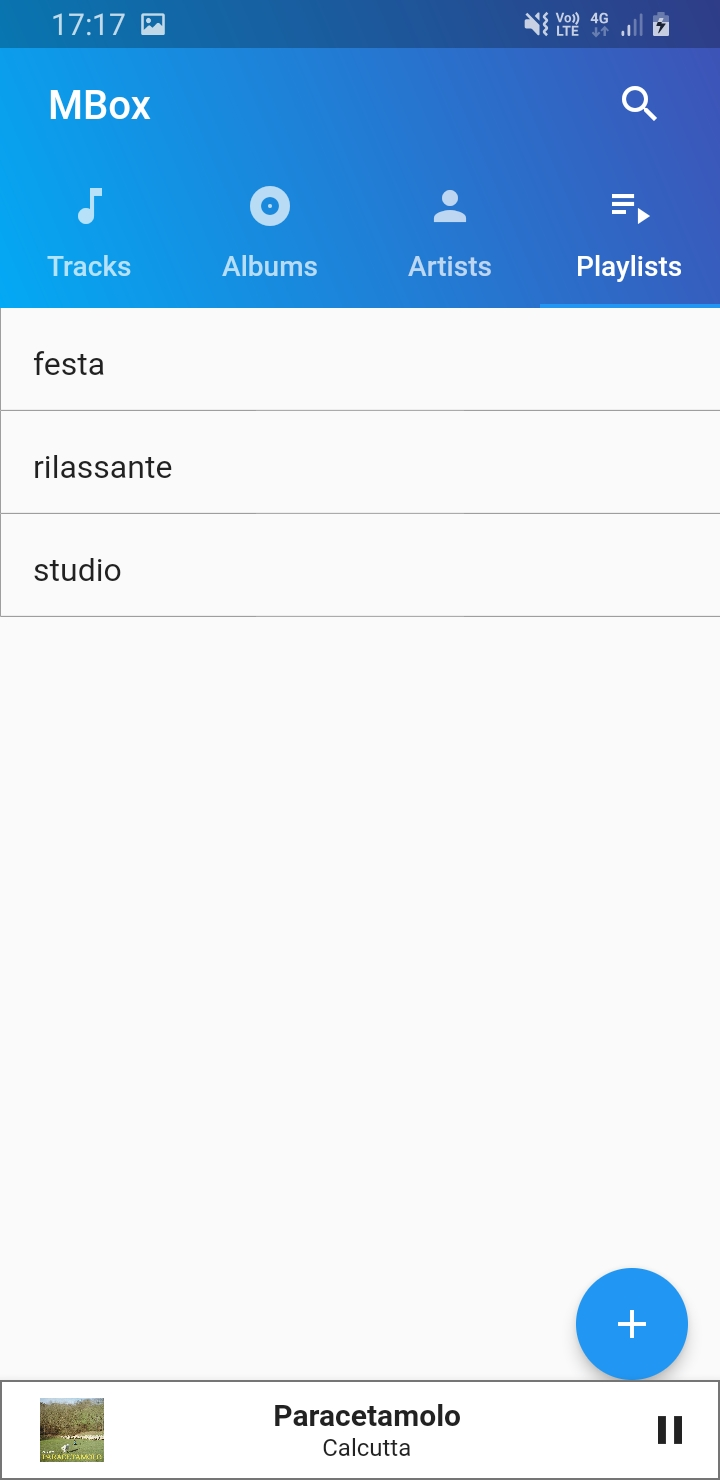
\includegraphics[width = 1.5in]{screens/5. Playlists.jpg}} &
    \subfloat[PlayingTrack]{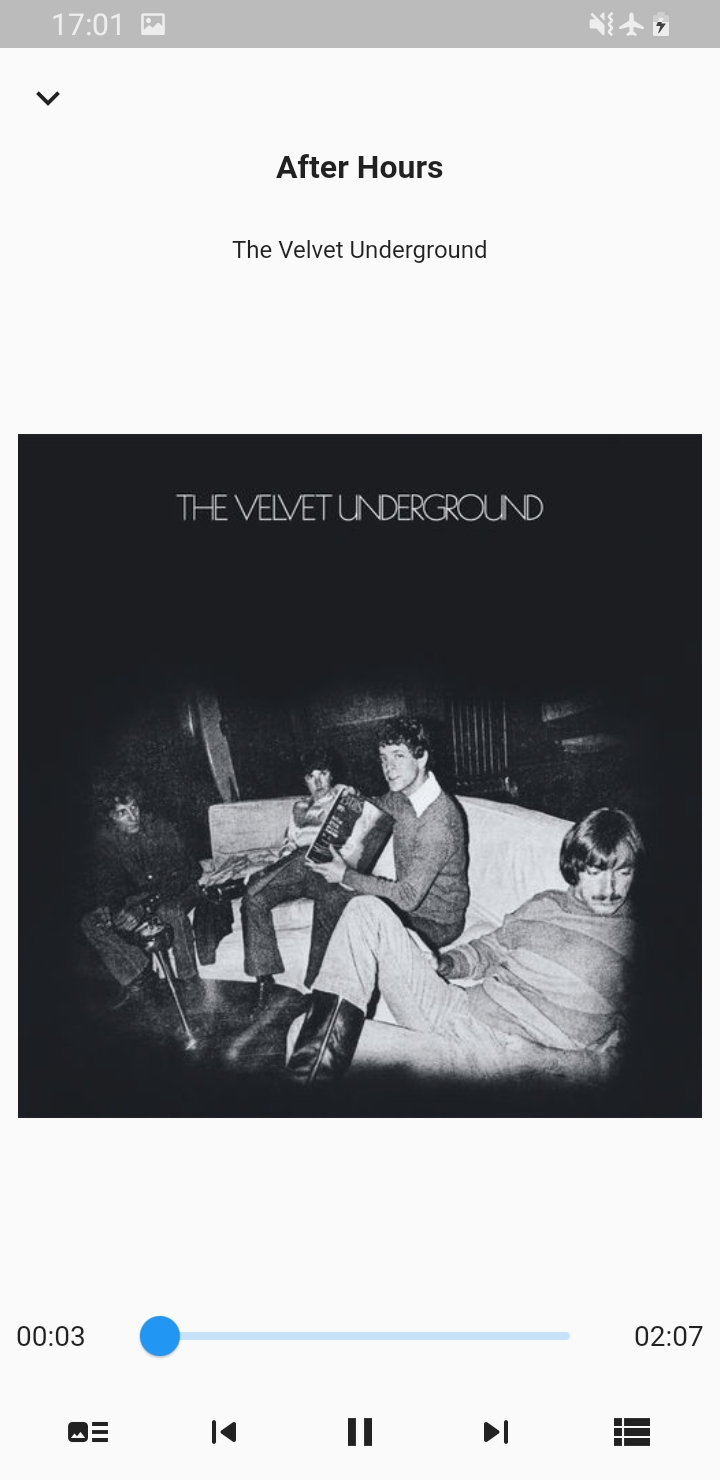
\includegraphics[width = 1.5in]{screens/6. PlayingTrack.jpg}}\\
    \\\\
    \subfloat[PlayingTrack with lyrics]{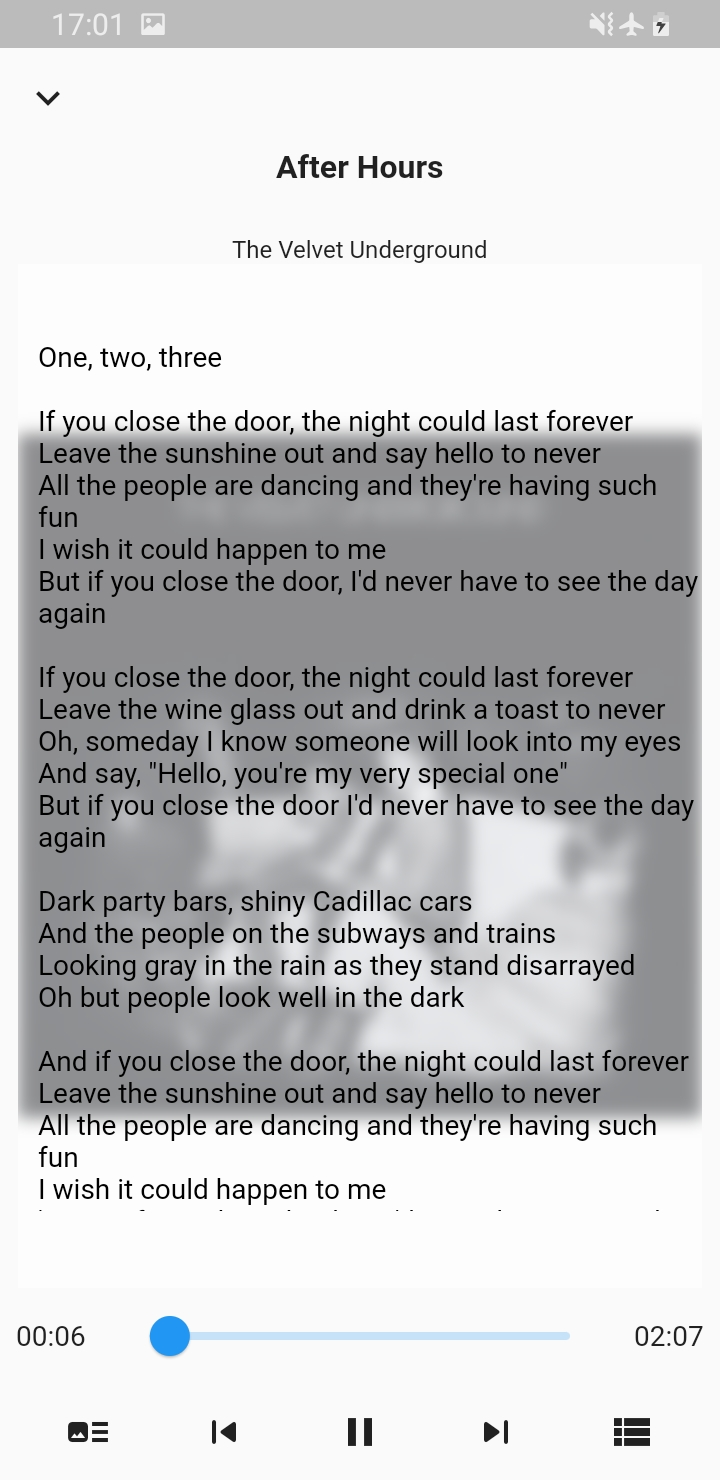
\includegraphics[width = 1.5in]{screens/7. Lyrics.jpg}} &
    \subfloat[ArtistInfo]{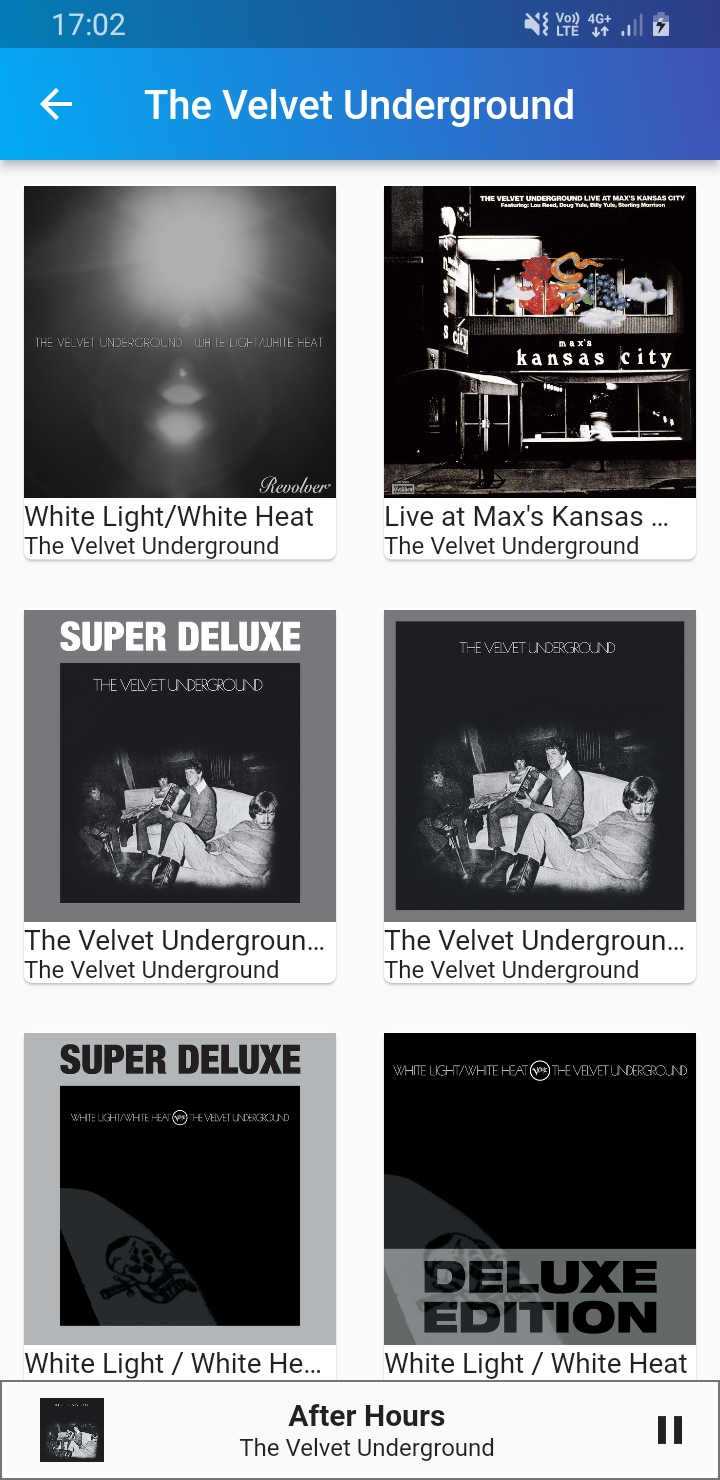
\includegraphics[width = 1.5in]{screens/8. ArtistInfo.jpg}}
    \end{tabular}
\end{figure}

\newpage
\begin{figure}[H]
    \begin{tabular}{cc}
    \subfloat[AlbumInfo]{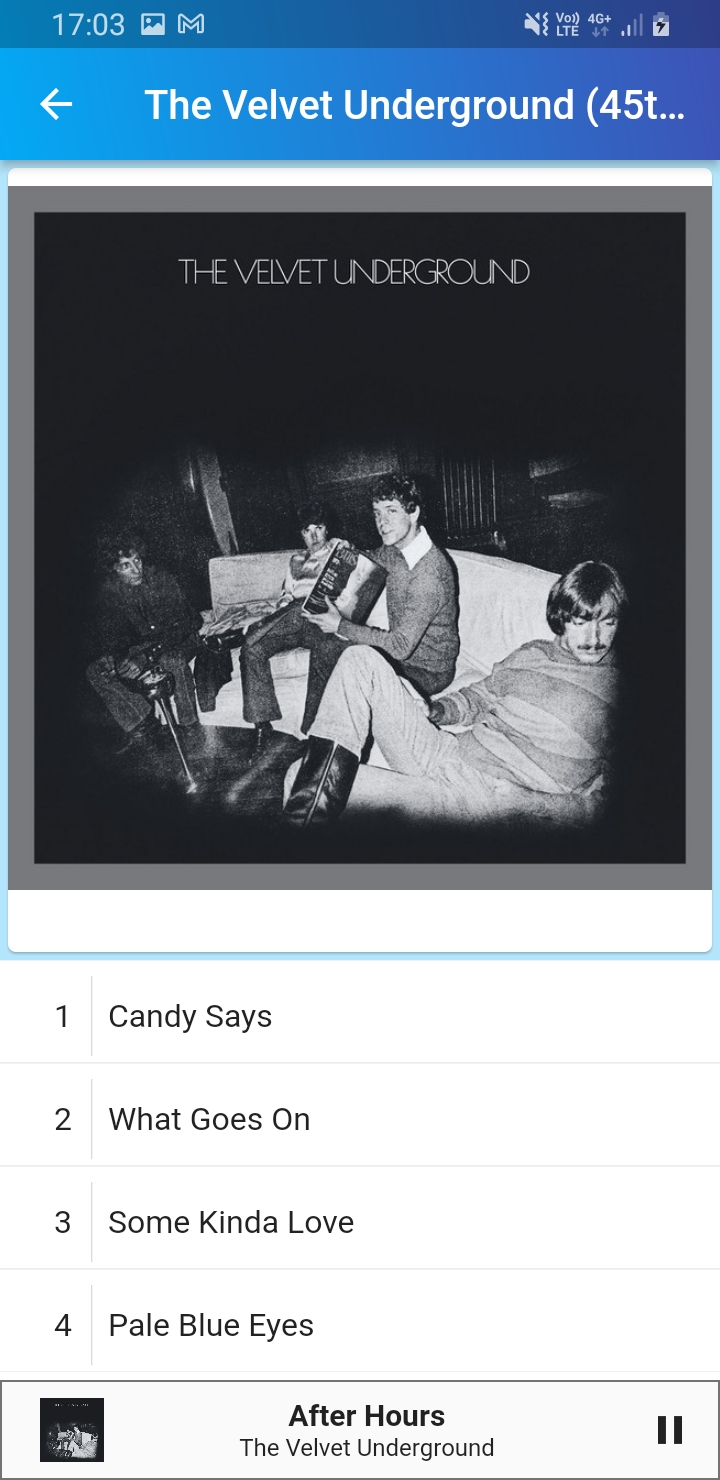
\includegraphics[width = 1.5in]{screens/9. AlbumInfo.jpg}}&
    \subfloat[AlbumTracks]{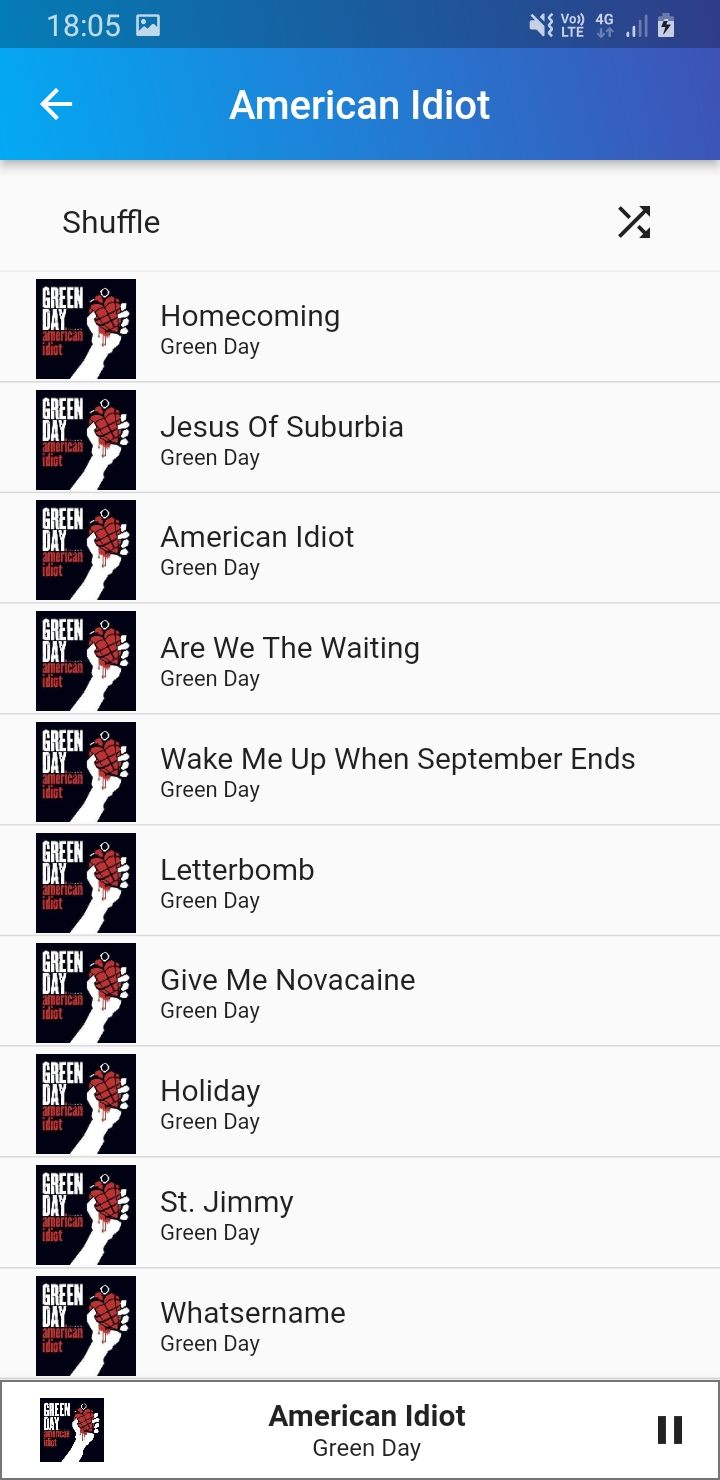
\includegraphics[width = 1.5in]{screens/10. AlbumTracks.jpg}}\\
    \\\\
    \subfloat[ArtistAlbums]{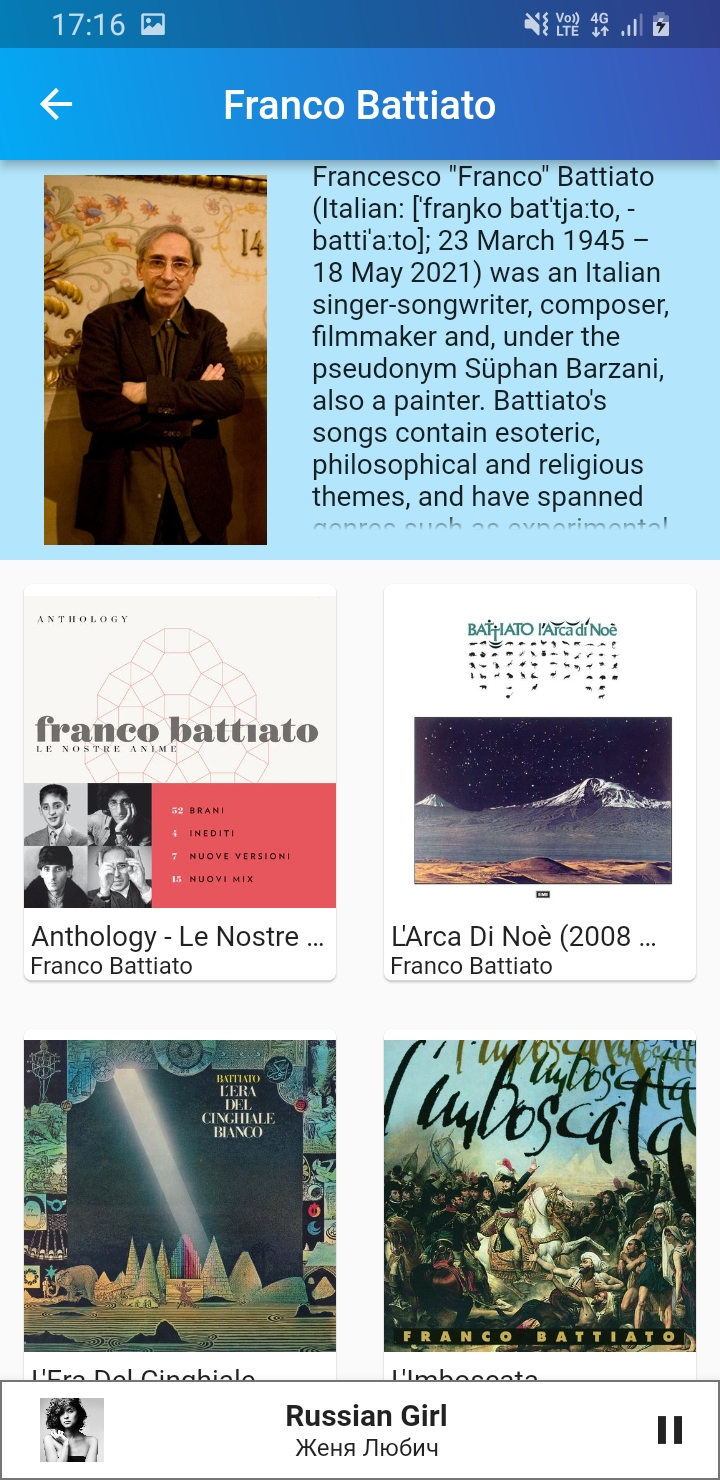
\includegraphics[width = 1.5in]{screens/11. ArtistAlbums.jpg}} &
    \subfloat[ShowPlaylist]{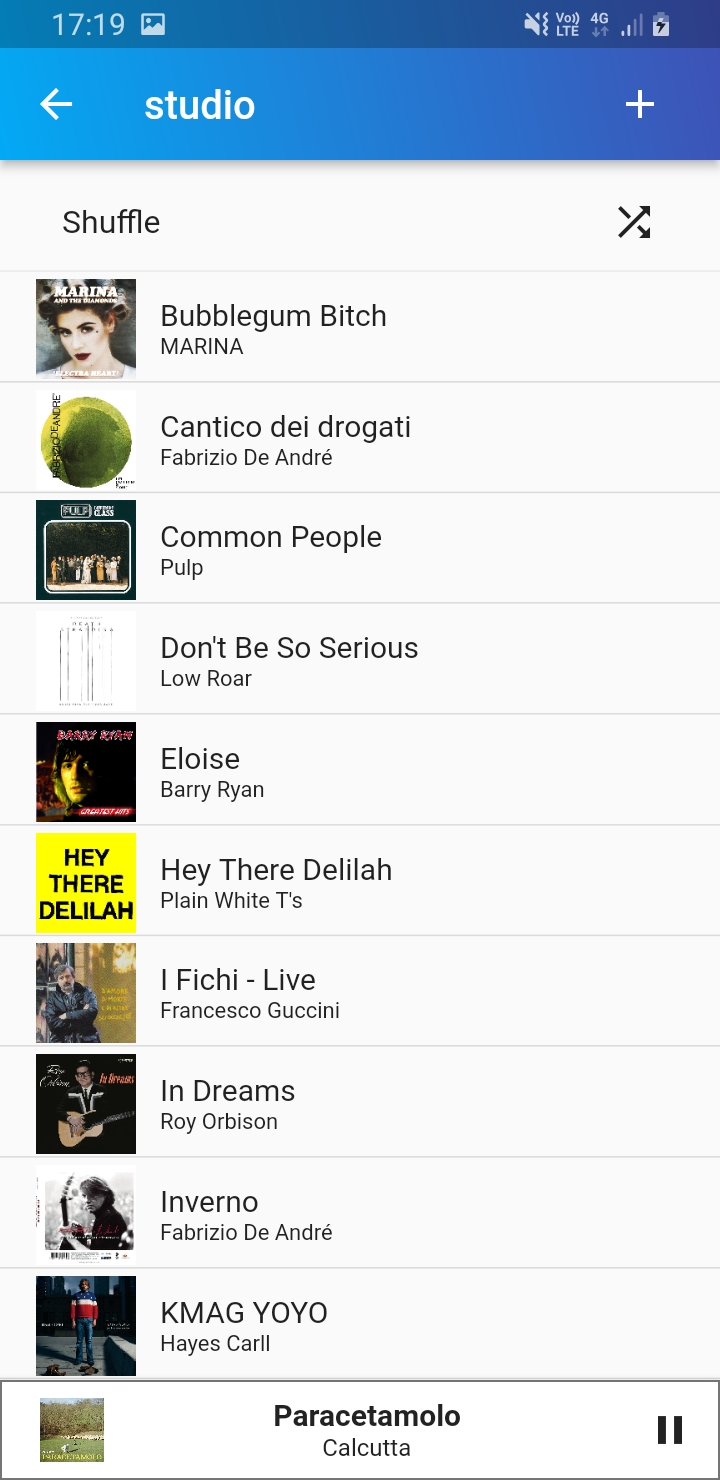
\includegraphics[width = 1.5in]{screens/12. ShowPlaylist.jpg}}
    \end{tabular}
\end{figure}

\newpage
\begin{figure}[H]
    \begin{tabular}{cc}
    \subfloat[SelectTracks]{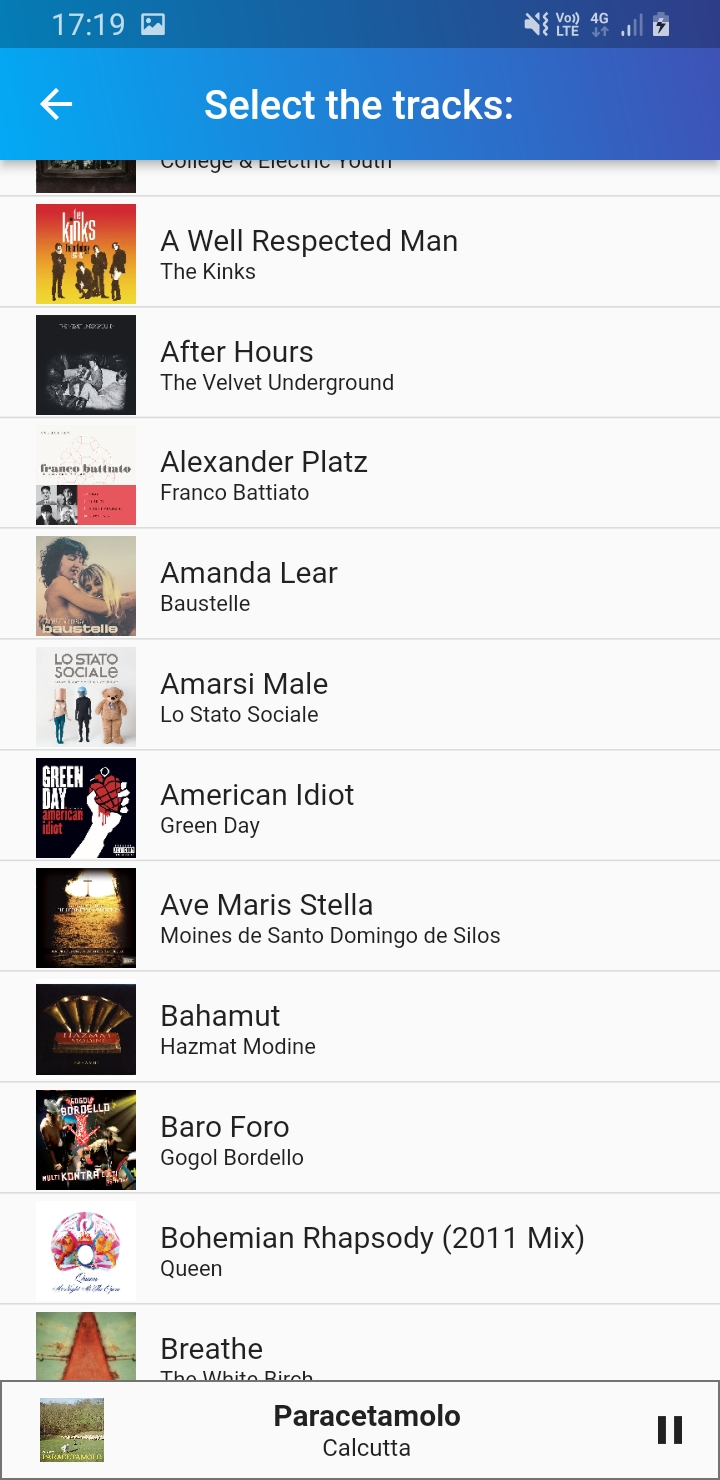
\includegraphics[width = 1.5in]{screens/13. SelectTracks.jpg}} &
    \subfloat[ShowQueue]{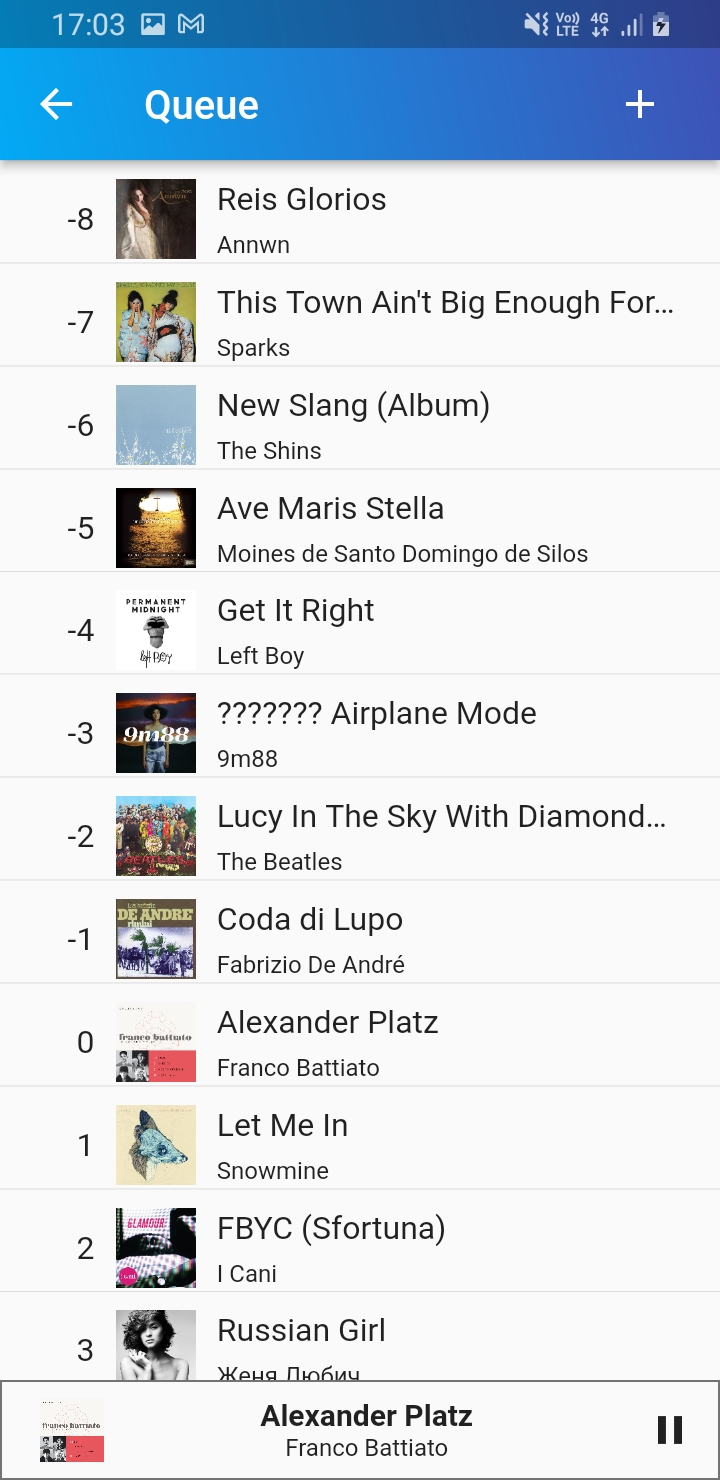
\includegraphics[width = 1.5in]{screens/14. ShowQueue.jpg}}\\
    \\\\
    \subfloat[SearchTracks / EditMetadata]{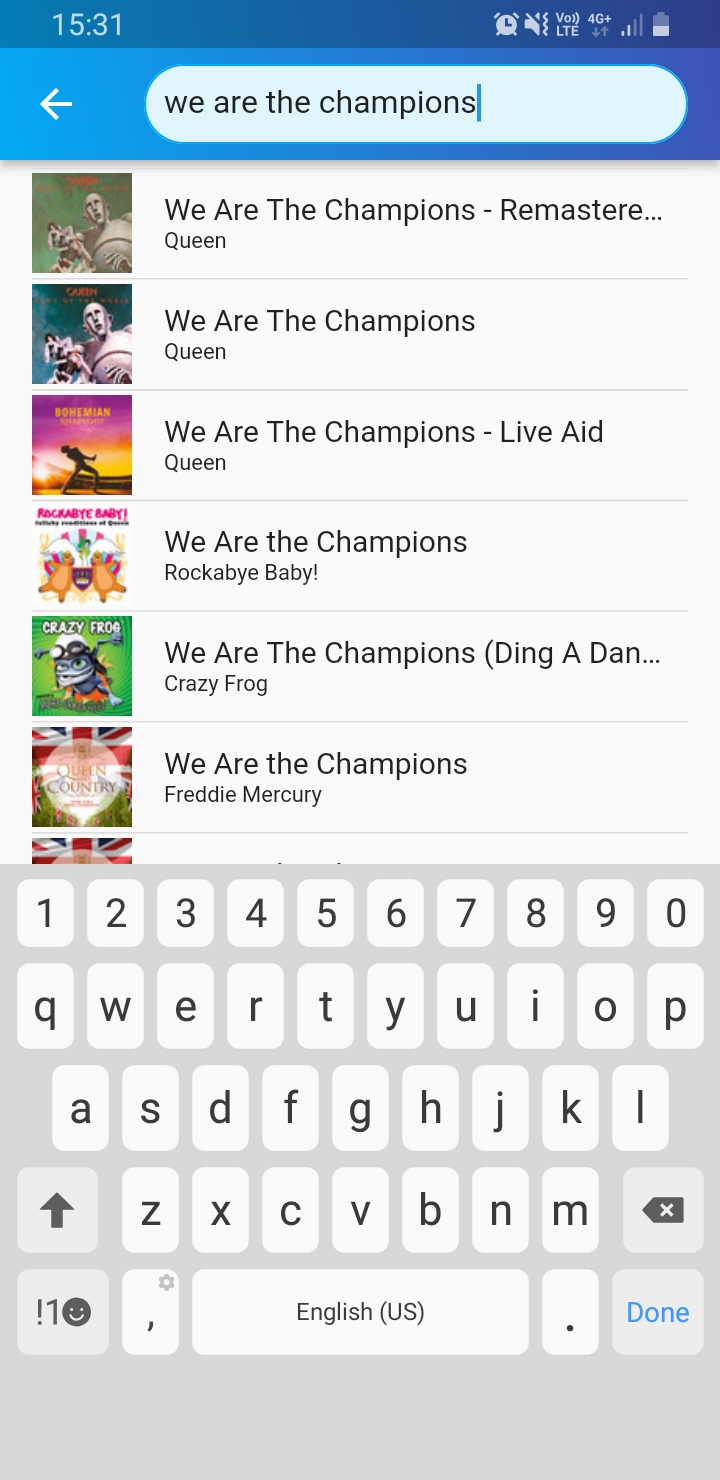
\includegraphics[width = 1.5in]{screens/21. SearchTracks.jpg}} &
    \subfloat[ArtistEditor]{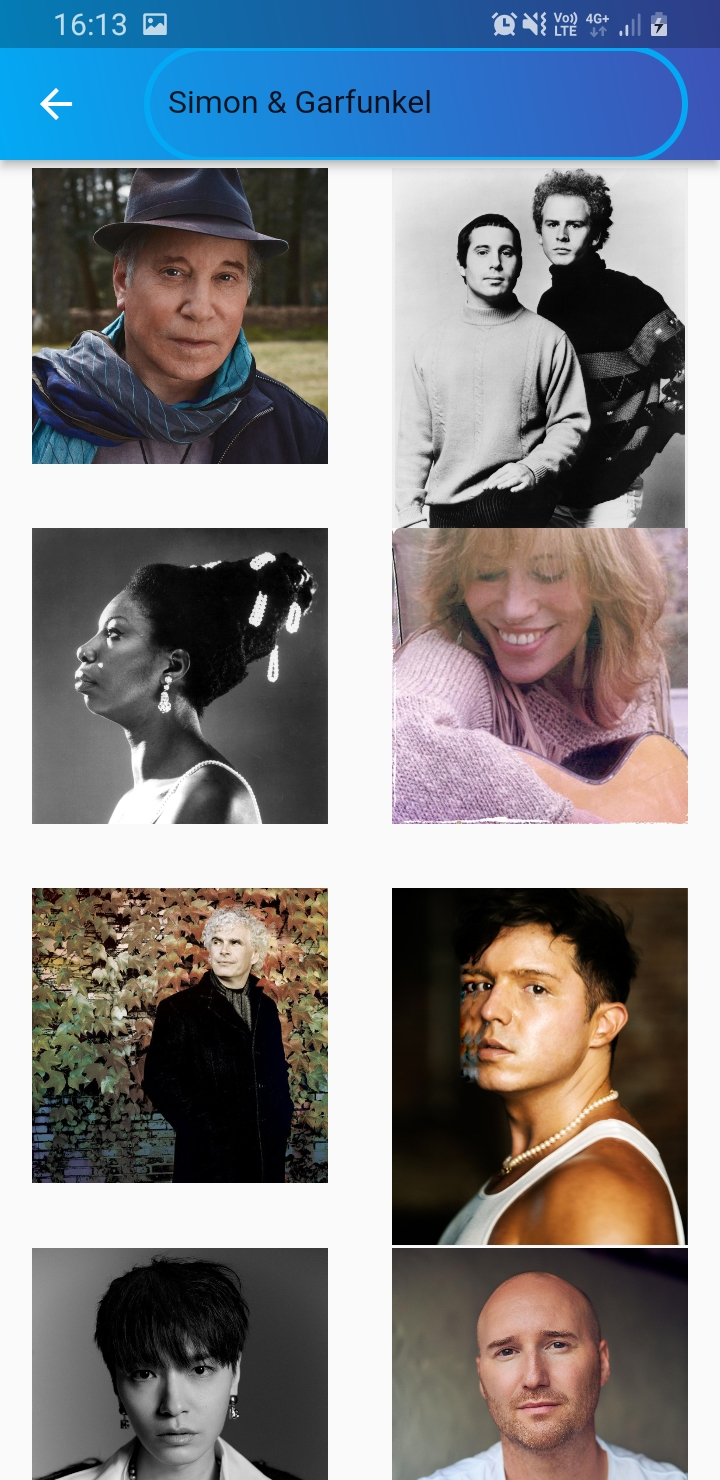
\includegraphics[width = 1.5in]{screens/22. ArtistEditor.jpg}}\\
    \end{tabular}
\end{figure}

\newpage

\begin{figure}[H]
    \subfloat[ciao]{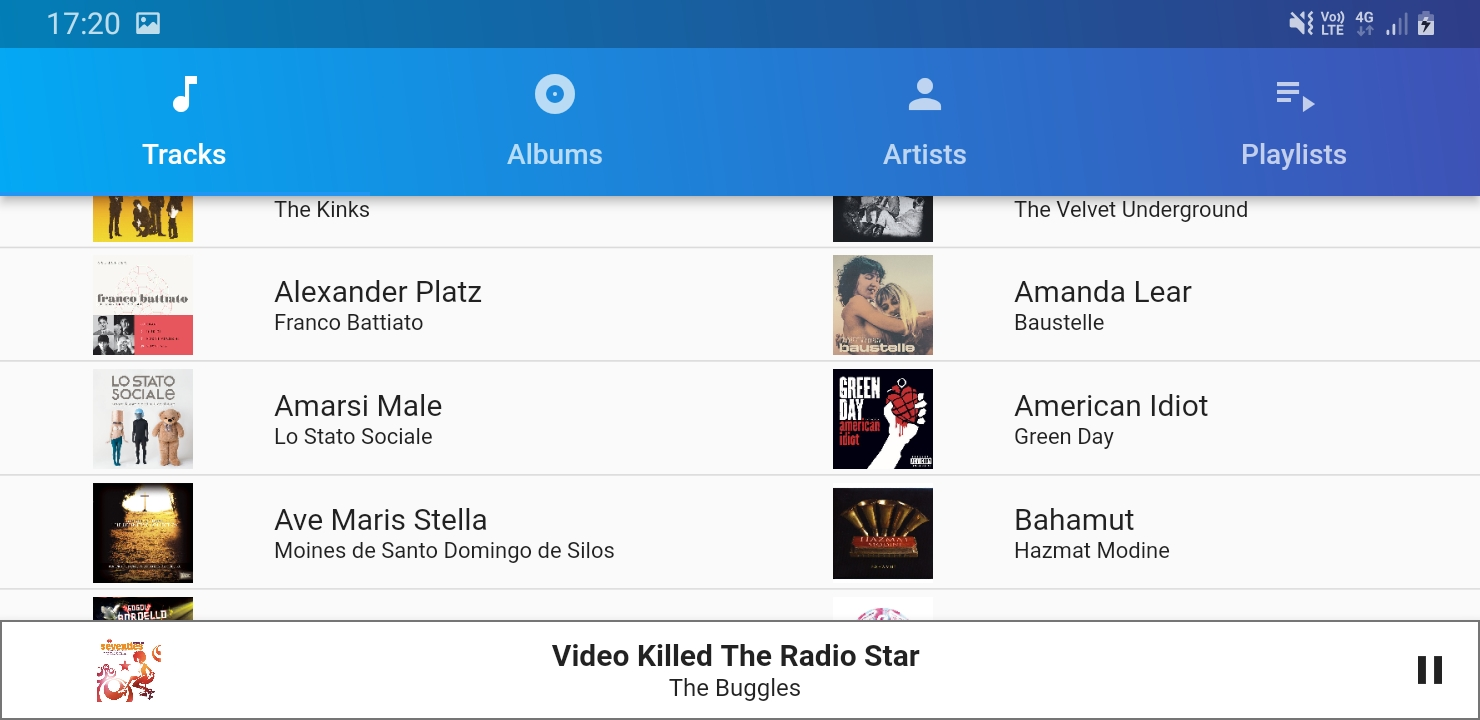
\includegraphics[width = 4.5in]{screens/15. Tracks_landscape.jpg}}\\\\
    \subfloat[ciao]{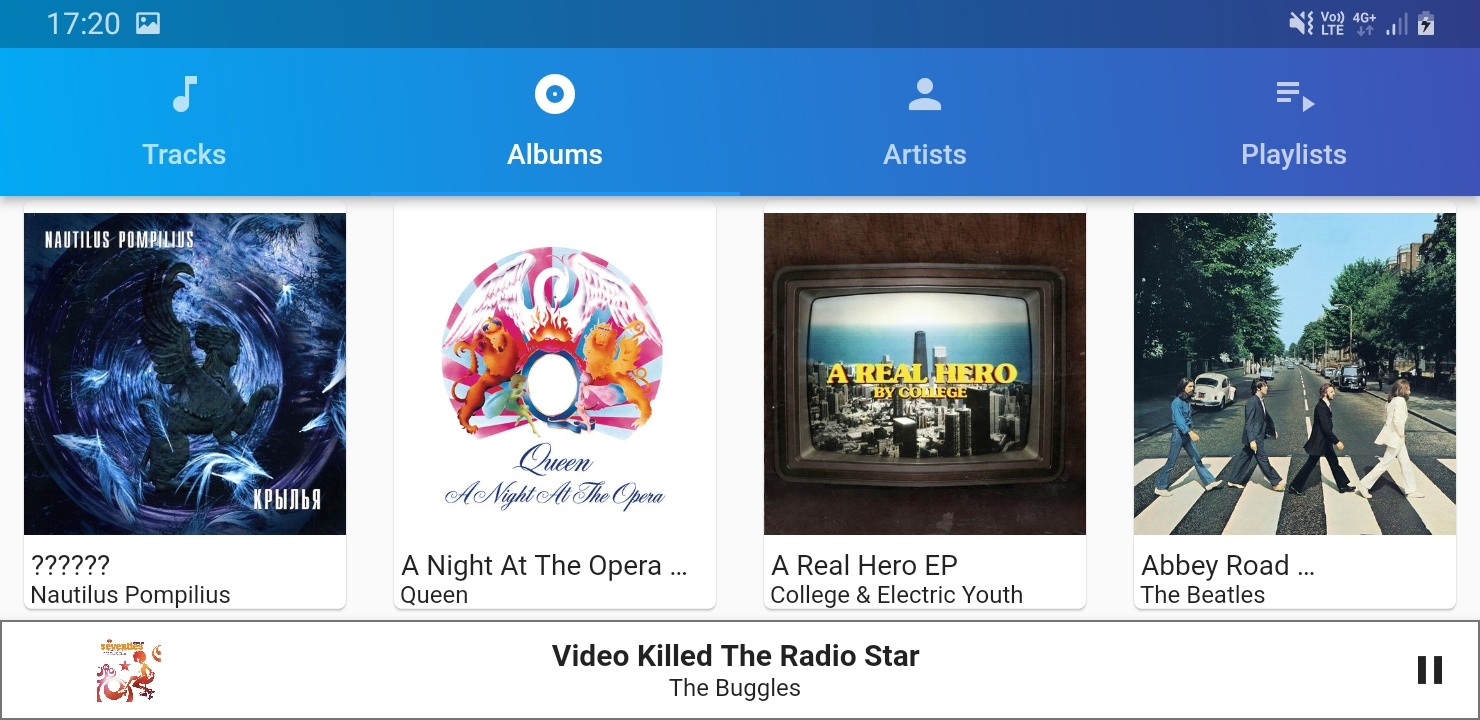
\includegraphics[width = 4.5in]{screens/16. Albums_landscape.jpg}}\\\\
    \subfloat[ciao]{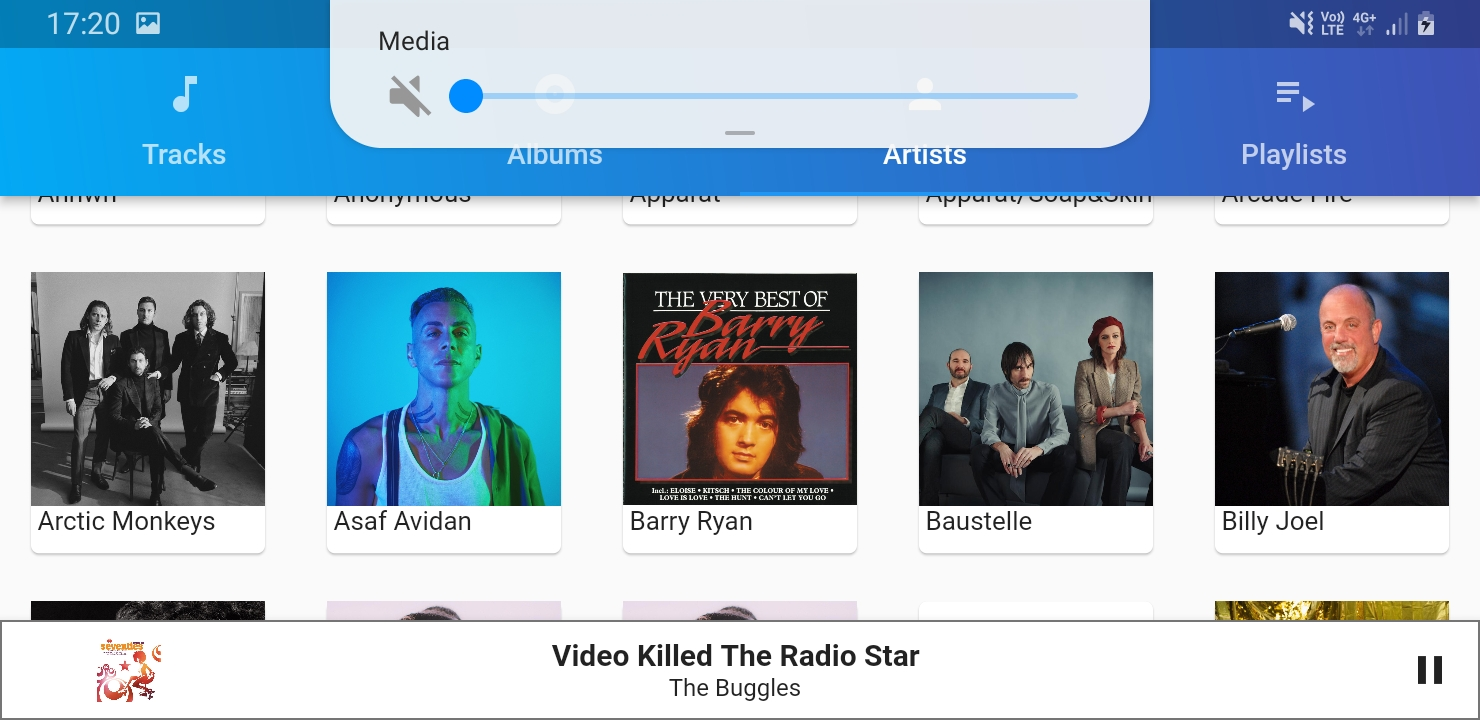
\includegraphics[width = 4.5in]{screens/17. Artists_landscape.jpg}}
\end{figure}

\newpage

\setcounter{subfigure}{19}
\begin{figure}[H]
    \subfloat[ciao]{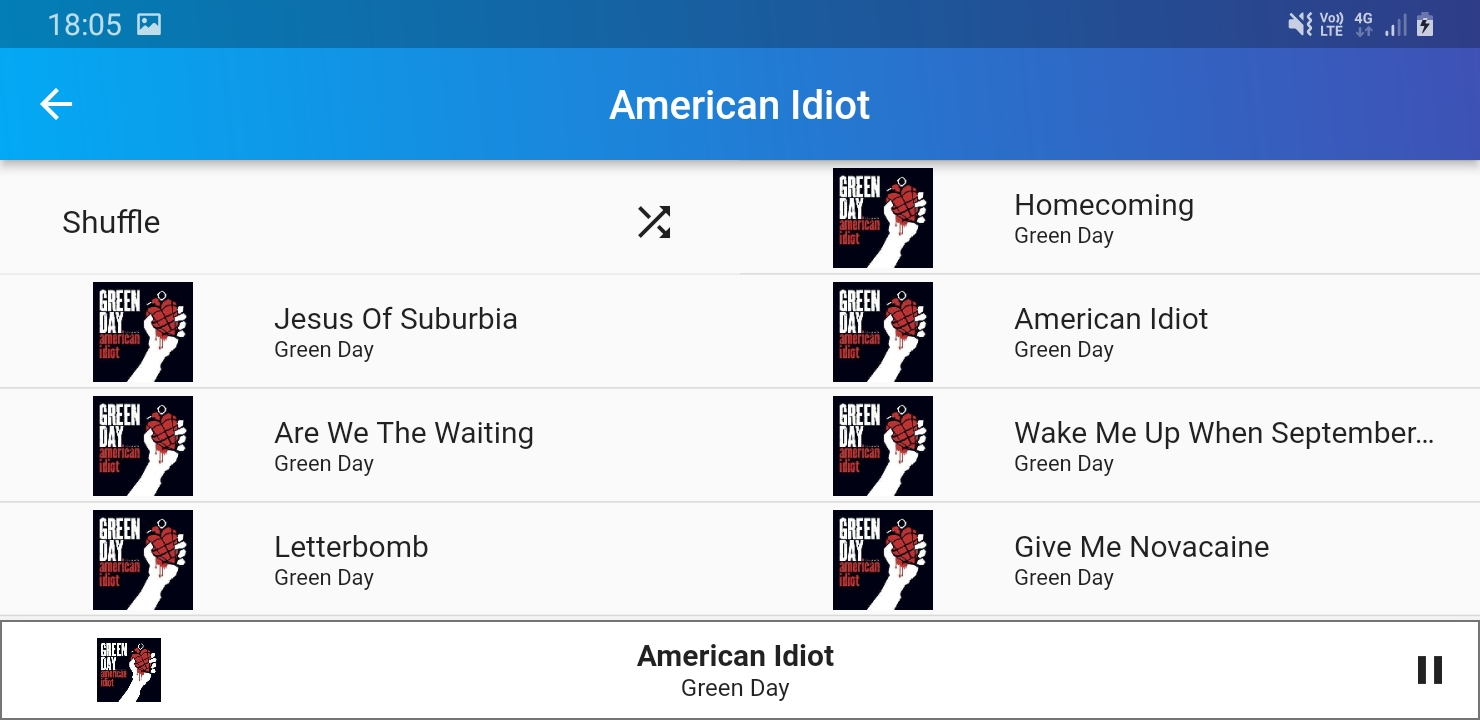
\includegraphics[width = 4.5in]{screens/18. AlbumTracks_landscape.jpg}}\\\\
    \subfloat[ciao]{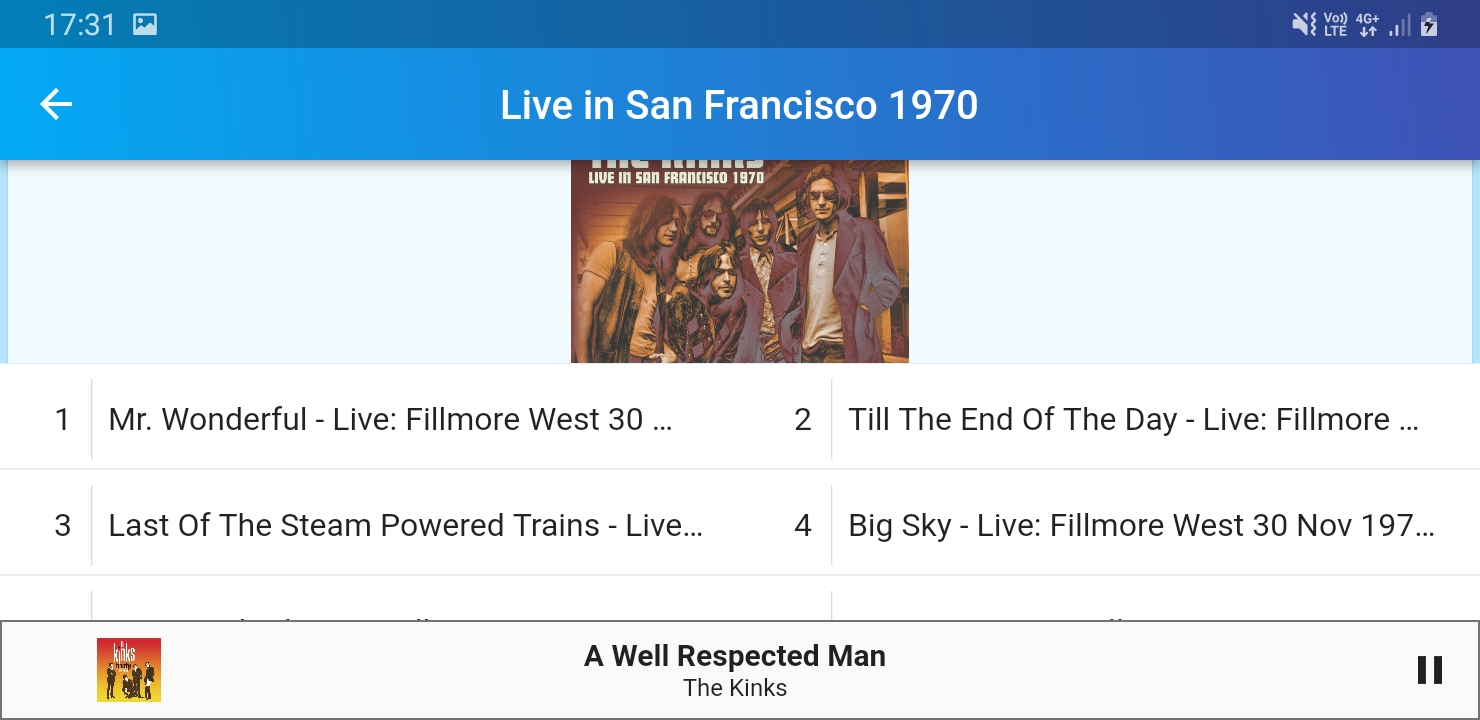
\includegraphics[width = 4.5in]{screens/19. AlbumInfo_landscape.jpg}}\\\\
    \subfloat[ciao]{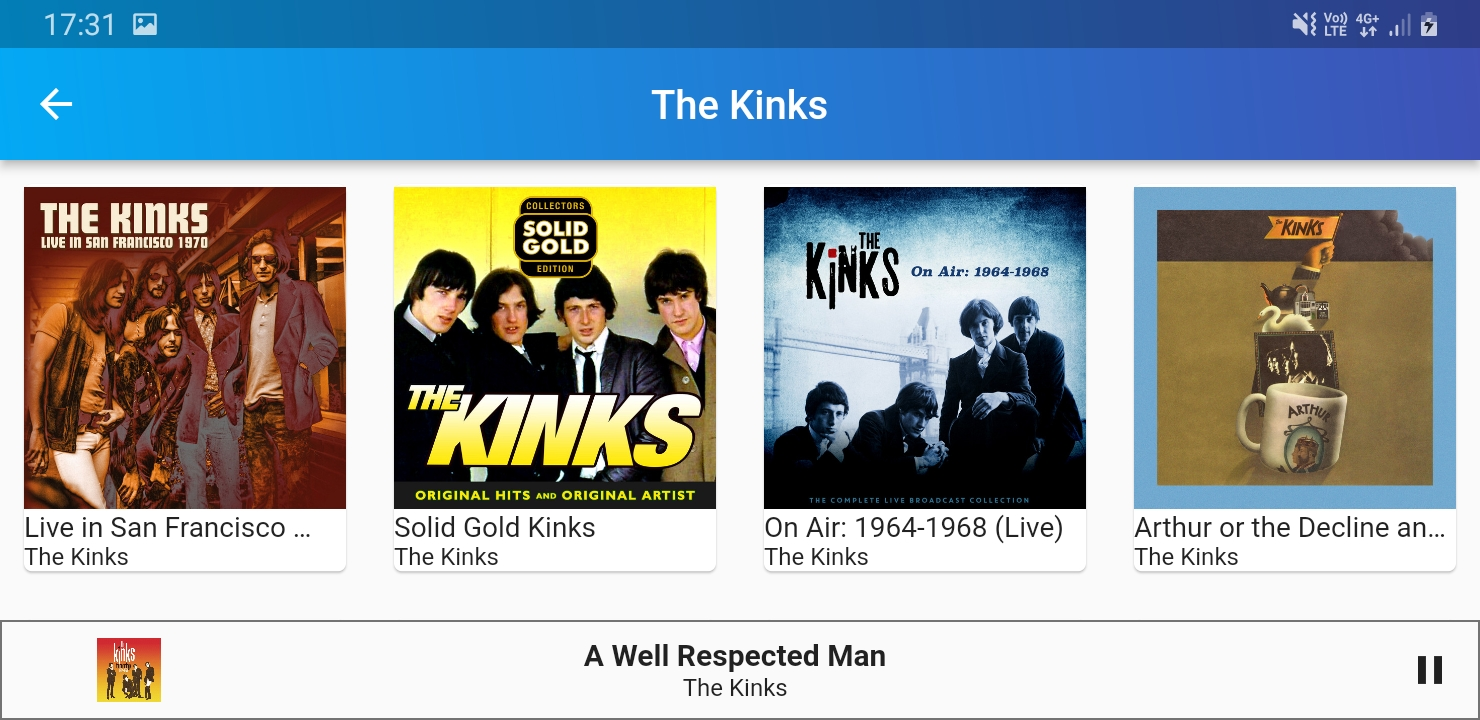
\includegraphics[width = 4.5in]{screens/20. ArtistInfo_landscape.jpg}}
\end{figure}

\newpage

\section{Implementation and Testing}

\subsection{Overview}
In this last section we provide all the necessary specifications about the
implementation and the testing of the system.
\\\\
This phase is, of course, critical for the development of a reliable software
system. It is important to observe that, while testing can show the presence of
bugs in the code, passing the tests does not imply the absence of errors in the
final application. Still, with our tests, we will try to find the majority of
the bugs before the product hits the market (and also after, maintenance is
important).

\subsection{Implementation}
For all the implementation processes we have chosen a \textbf{bottom-up}
approach, which consists in implementing first the base components, and then, in
a iterative way, those that require them. We topologically sort the dependencies
between the components such that every time we implement one of them we have
already realized all the others on which it depends.
\\\\
The unit testing has been carried out in parallel with the implementation. Using
the bottom-up approach we have used some drivers, during all testing process, to
mimic the behavior of the elements that use the component under test. On
the other hand, the selected approach does not require the creation of stubs,
elements that simulate the behavior of not yet implemented modules, required by
the component under test.
\\\\
With this incremental approach we have in each moment fully functional
components, being sure that the work already done is complete and functional.
Moreover, beginning from the bottom, the core components have been implemented
first, and so the ones that have been tested, improving the robustness of the
overall system.
\\\\
The first element that we have implemented is the \textbf{Database} component,
which manages the model, i.e. the data, of our application, and so it is
required by most of the components of the system.
\\\\
At this point we can implement the \textbf{Loader} component; this component is essential
for the rest of the application, since it provides all the information obtained
from the internet, so we implement it right after the Database.
\\\\
The \textbf{Player} provides core functionalities to the rest of the application
and must be implemented as soon as the Database and the Loader are completed,
because it depends heavily on them.
\\\\
With these components the core of the application is ready even if there is no
graphical interface to access it yet. Before we move to the frontend components,
we can implement the \textbf{Worker} to improve the performance of
the Database.
\\\\
For the components of the user interface we implement first the \textbf{Home}
screen, and shortly after the tabs it holds: \textbf{Tracks}, \textbf{Albums},
\textbf{Artists}, \textbf{Playlists}. After these, we implement the
\textbf{PlayingTrack} screen. Indeed this is the center of the application and
the other peripherical screens can now be implemented.
\\\\
We can now implement all the remaining screen following a bottom up order:
\begin{enumerate}
    \item \textbf{ArtistInfo} and \textbf{ShowQueue}
    \item \textbf{AlbumInfo} and \textbf{SelectTracks}
    \item \textbf{SearchSong} and \textbf{MetadataEditor}
\end{enumerate}

\subsection{Testing}
As we develop the system we have to check that all functional and non functional
requirements have are met. In particular for the backend components some tests
have been devised so to check that the core offered features work as expected.
The Database, Worker, Loader are unit tested with automatic testing. Integration
tests for the backend have been developed to check that the components work
together correctly.
\\\\
For what concerns the frontend part automatic testing is very hard to implement,
since it would consits in checking regressions in GUI. So for checking that the
screens are correct we save the GUI appearance in a particular state and then we
visually check that changes to the code do not introduce regression errors.


\end{document}
